\documentclass[aspectratio=169,10pt]{beamer}

% Modern professional theme
\usetheme{metropolis}
\usecolortheme{default}

% Custom color scheme
\definecolor{primaryblue}{RGB}{20,75,140}
\definecolor{secondaryblue}{RGB}{70,130,180}
\definecolor{accentorange}{RGB}{230,95,45}
\definecolor{lightgray}{RGB}{245,245,245}
\definecolor{darkgray}{RGB}{45,45,45}

% Metropolis color customization
\setbeamercolor{progress bar}{fg=primaryblue,bg=lightgray}
\setbeamercolor{title separator}{fg=primaryblue}
\setbeamercolor{progress bar in head/foot}{fg=primaryblue}
\setbeamercolor{progress bar in section page}{fg=primaryblue}
\setbeamercolor{frametitle}{bg=primaryblue,fg=white}
\setbeamercolor{title}{fg=primaryblue}
\setbeamercolor{subtitle}{fg=secondaryblue}
\setbeamercolor{structure}{fg=primaryblue}
\setbeamercolor{alerted text}{fg=accentorange}
\setbeamercolor{block title}{bg=primaryblue,fg=white}
\setbeamercolor{block body}{bg=lightgray,fg=darkgray}
\setbeamercolor{block title alerted}{bg=accentorange,fg=white}
\setbeamercolor{block body alerted}{bg=lightgray,fg=darkgray}

% Packages
\usepackage{amsmath,amssymb,amsfonts}
\usepackage{graphicx}
\usepackage{booktabs}
\usepackage{xcolor}
\usepackage{tikz}

% Professional formatting
\setbeamertemplate{navigation symbols}{}
\setbeamertemplate{footline}[frame number]

% Title information
\title{Computer Vision \& Deep Learning II}
\subtitle{CMSC 178IP - Digital Image Processing}
\author{Noel Jeffrey Pinton}
\institute{University of the Philippines - Cebu\\Department of Computer Science}
\date{}

% Adjust title page spacing
\setbeamertemplate{title page}[default][colsep=-4bp,rounded=true]

\begin{document}

% Title slide
\begin{frame}
\titlepage
\end{frame}

% Table of contents
\begin{frame}{Course Outline}
\tableofcontents
\end{frame}

\section{Image Classification}

\begin{frame}{Image Classification Overview}
\begin{alertblock}{Definition}
Image classification assigns a single label to an entire image from a predefined set of categories.
\end{alertblock}

\textbf{Core Task:}
\begin{itemize}
\item Input: Image $\mathbf{I} \in \mathbb{R}^{H \times W \times C}$
\item Output: Class label $y \in \{1, 2, \ldots, K\}$
\item Goal: Learn mapping $f: \mathbf{I} \rightarrow y$
\end{itemize}

\textbf{Applications:}
\begin{itemize}
\item Medical diagnosis (X-ray, MRI classification)
\item Quality control in manufacturing
\item Content moderation and filtering
\item Autonomous vehicles (traffic sign recognition)
\end{itemize}
\end{frame}

\begin{frame}{MNIST Dataset}
\begin{columns}
\column{0.55\textwidth}
\textbf{Dataset Properties:}
\begin{itemize}
\item 70,000 handwritten digits (0-9)
\item 60,000 training, 10,000 test images
\item 28×28 grayscale images
\item Centered and size-normalized
\end{itemize}

\textbf{Challenges:}
\begin{itemize}
\item Writing style variations
\item Digit similarity (1 vs 7, 3 vs 8)
\item Image noise and artifacts
\end{itemize}

\column{0.4\textwidth}
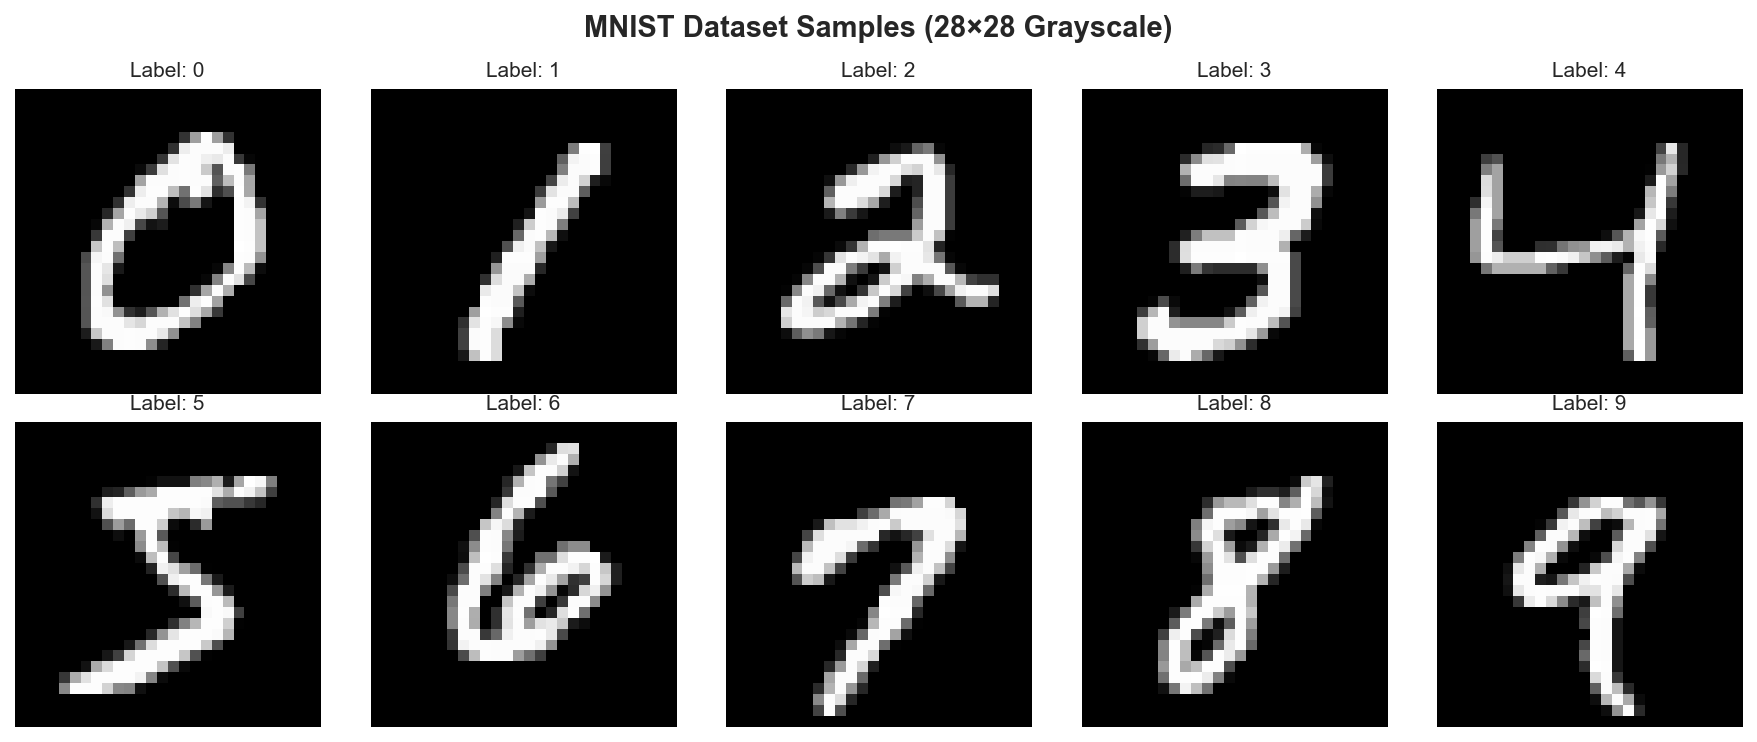
\includegraphics[width=\textwidth]{../figures/mnist_samples.png}
\centering{\small Sample MNIST digits}
\end{columns}
\end{frame}

\begin{frame}{CIFAR-10 Dataset}
\begin{columns}
\column{0.55\textwidth}
\textbf{Dataset Properties:}
\begin{itemize}
\item 60,000 color images in 10 classes
\item 50,000 training, 10,000 test
\item 32×32 RGB images
\item Real-world natural images
\end{itemize}

\textbf{Classes:}
\begin{itemize}
\item Airplane, Automobile, Bird, Cat, Deer
\item Dog, Frog, Horse, Ship, Truck
\end{itemize}

\column{0.4\textwidth}
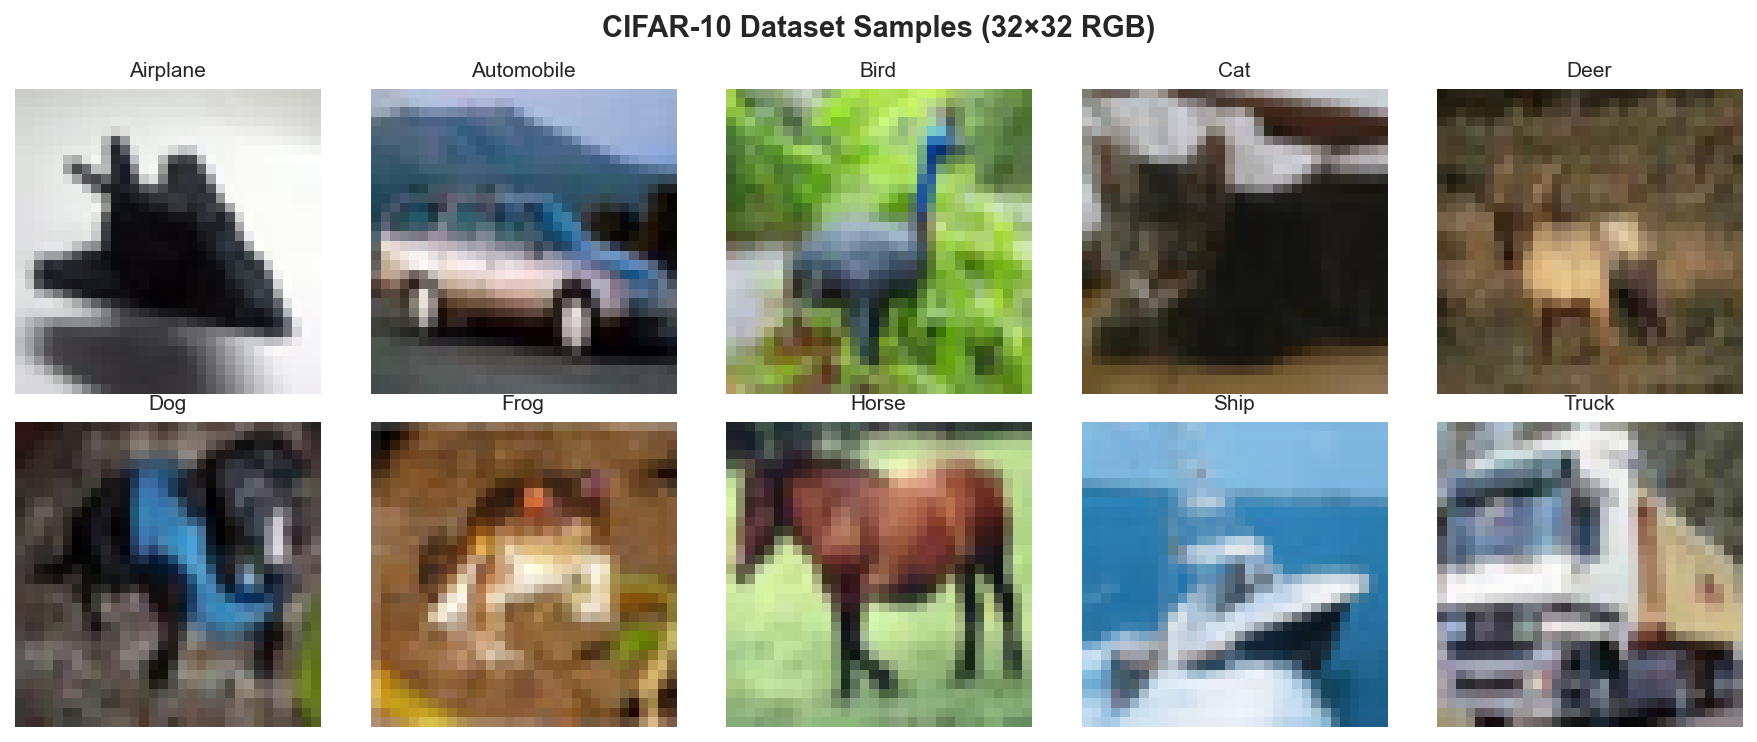
\includegraphics[width=\textwidth]{../figures/cifar10_samples.png}
\centering{\small CIFAR-10 examples}
\end{columns}
\end{frame}

\begin{frame}{CNN Architecture for Classification}
\begin{center}
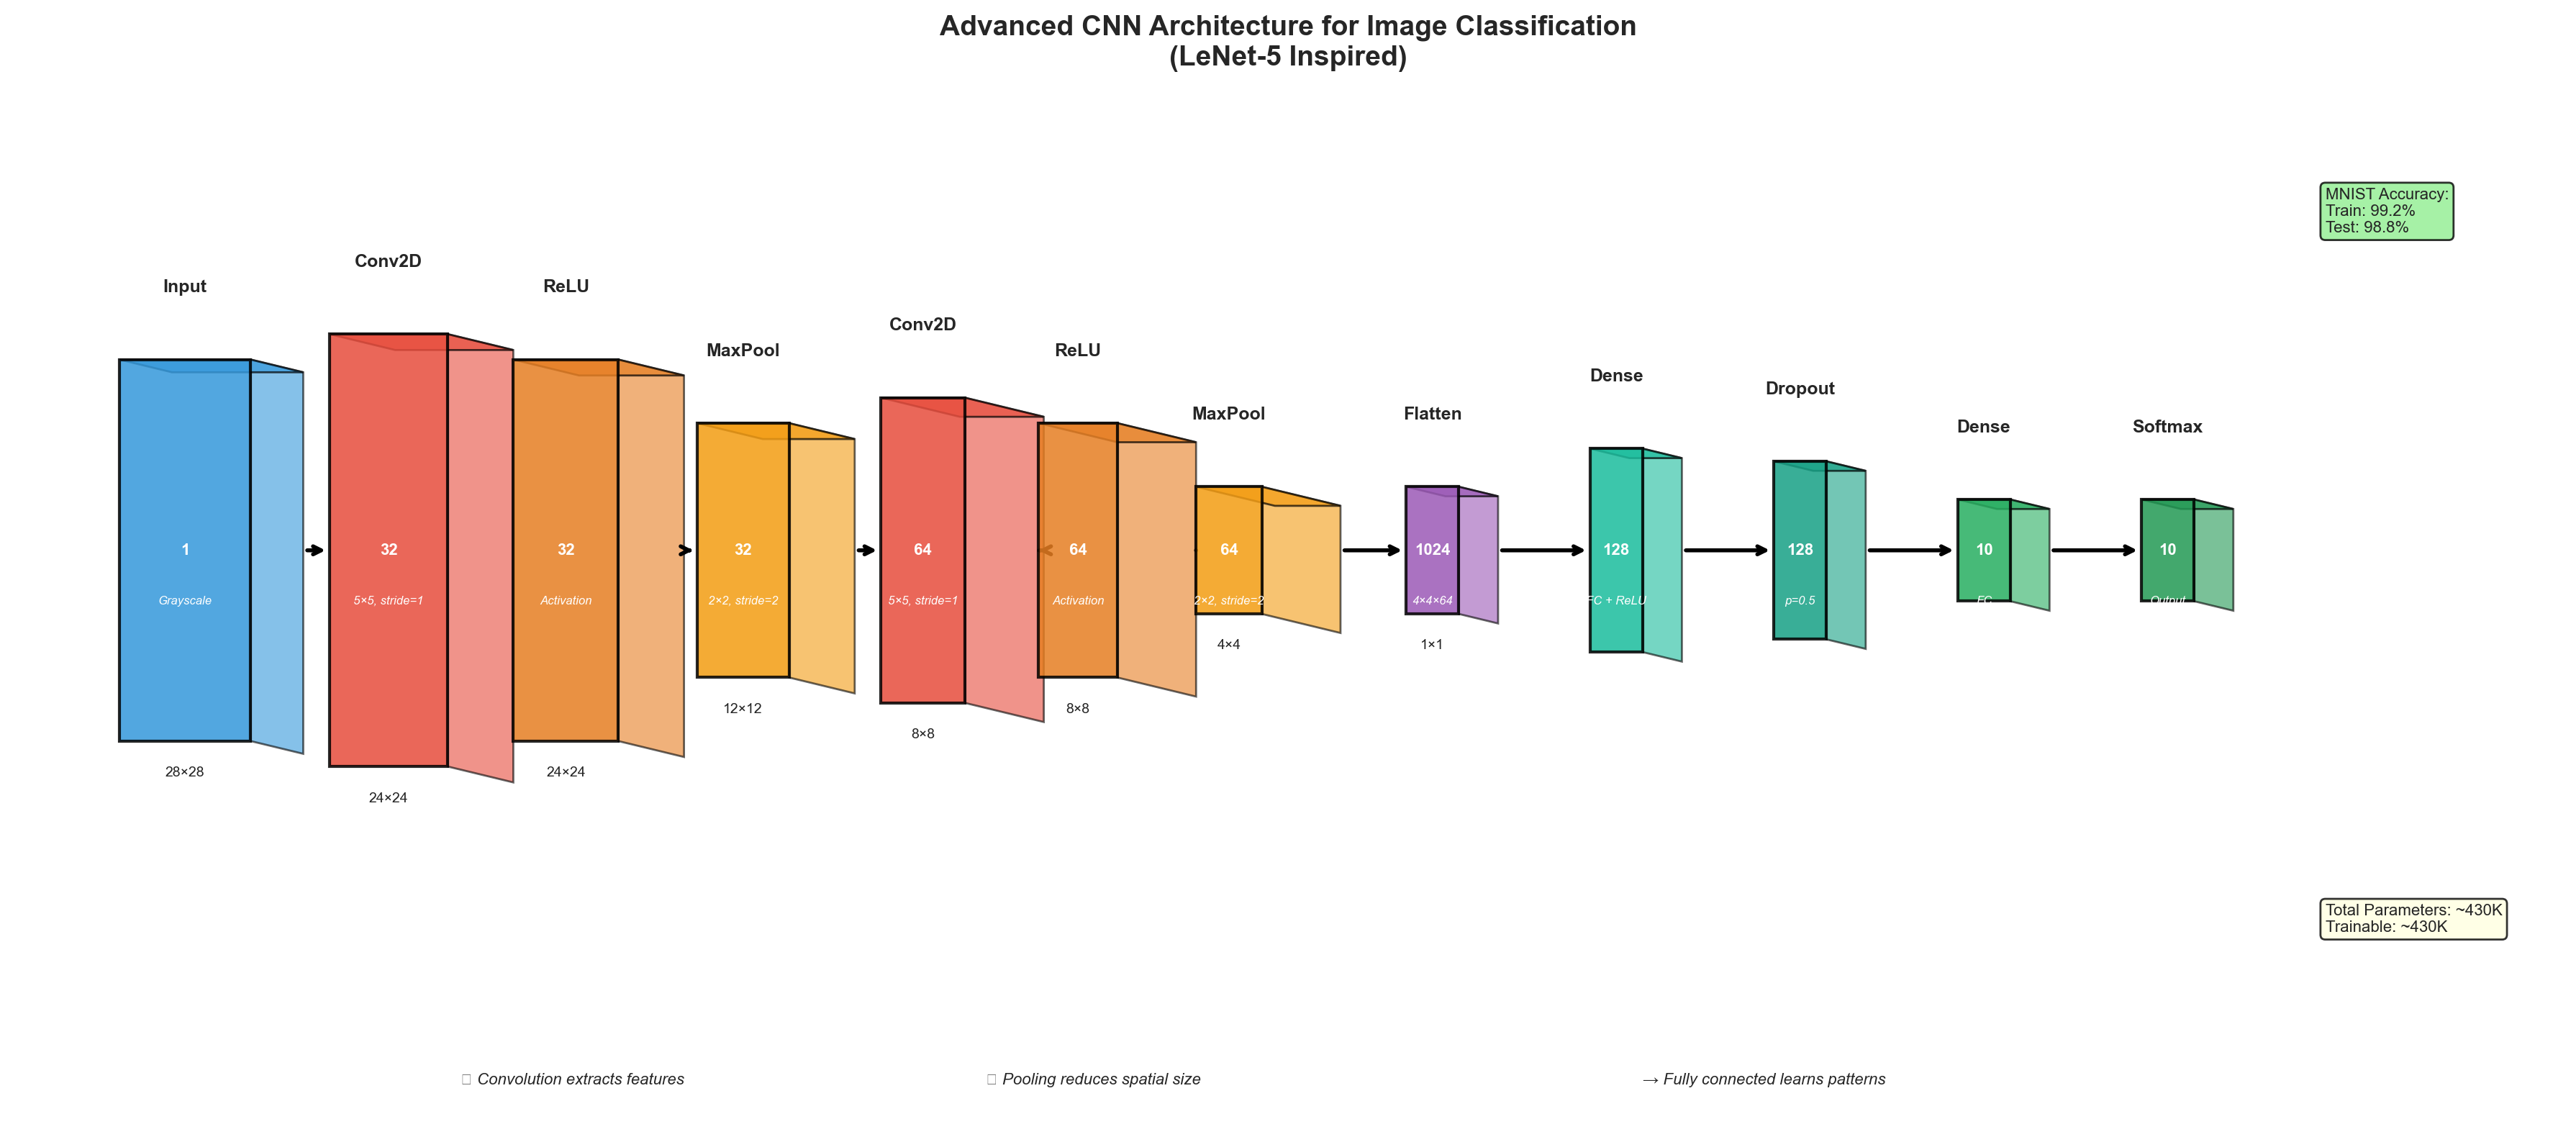
\includegraphics[width=0.85\textwidth]{../figures/cnn_architecture.png}
\end{center}

\textbf{Components:} Conv (features) → Pool (downsample) → FC (classify) → Softmax
\end{frame}

\begin{frame}{Feature Map Visualization}
\begin{center}
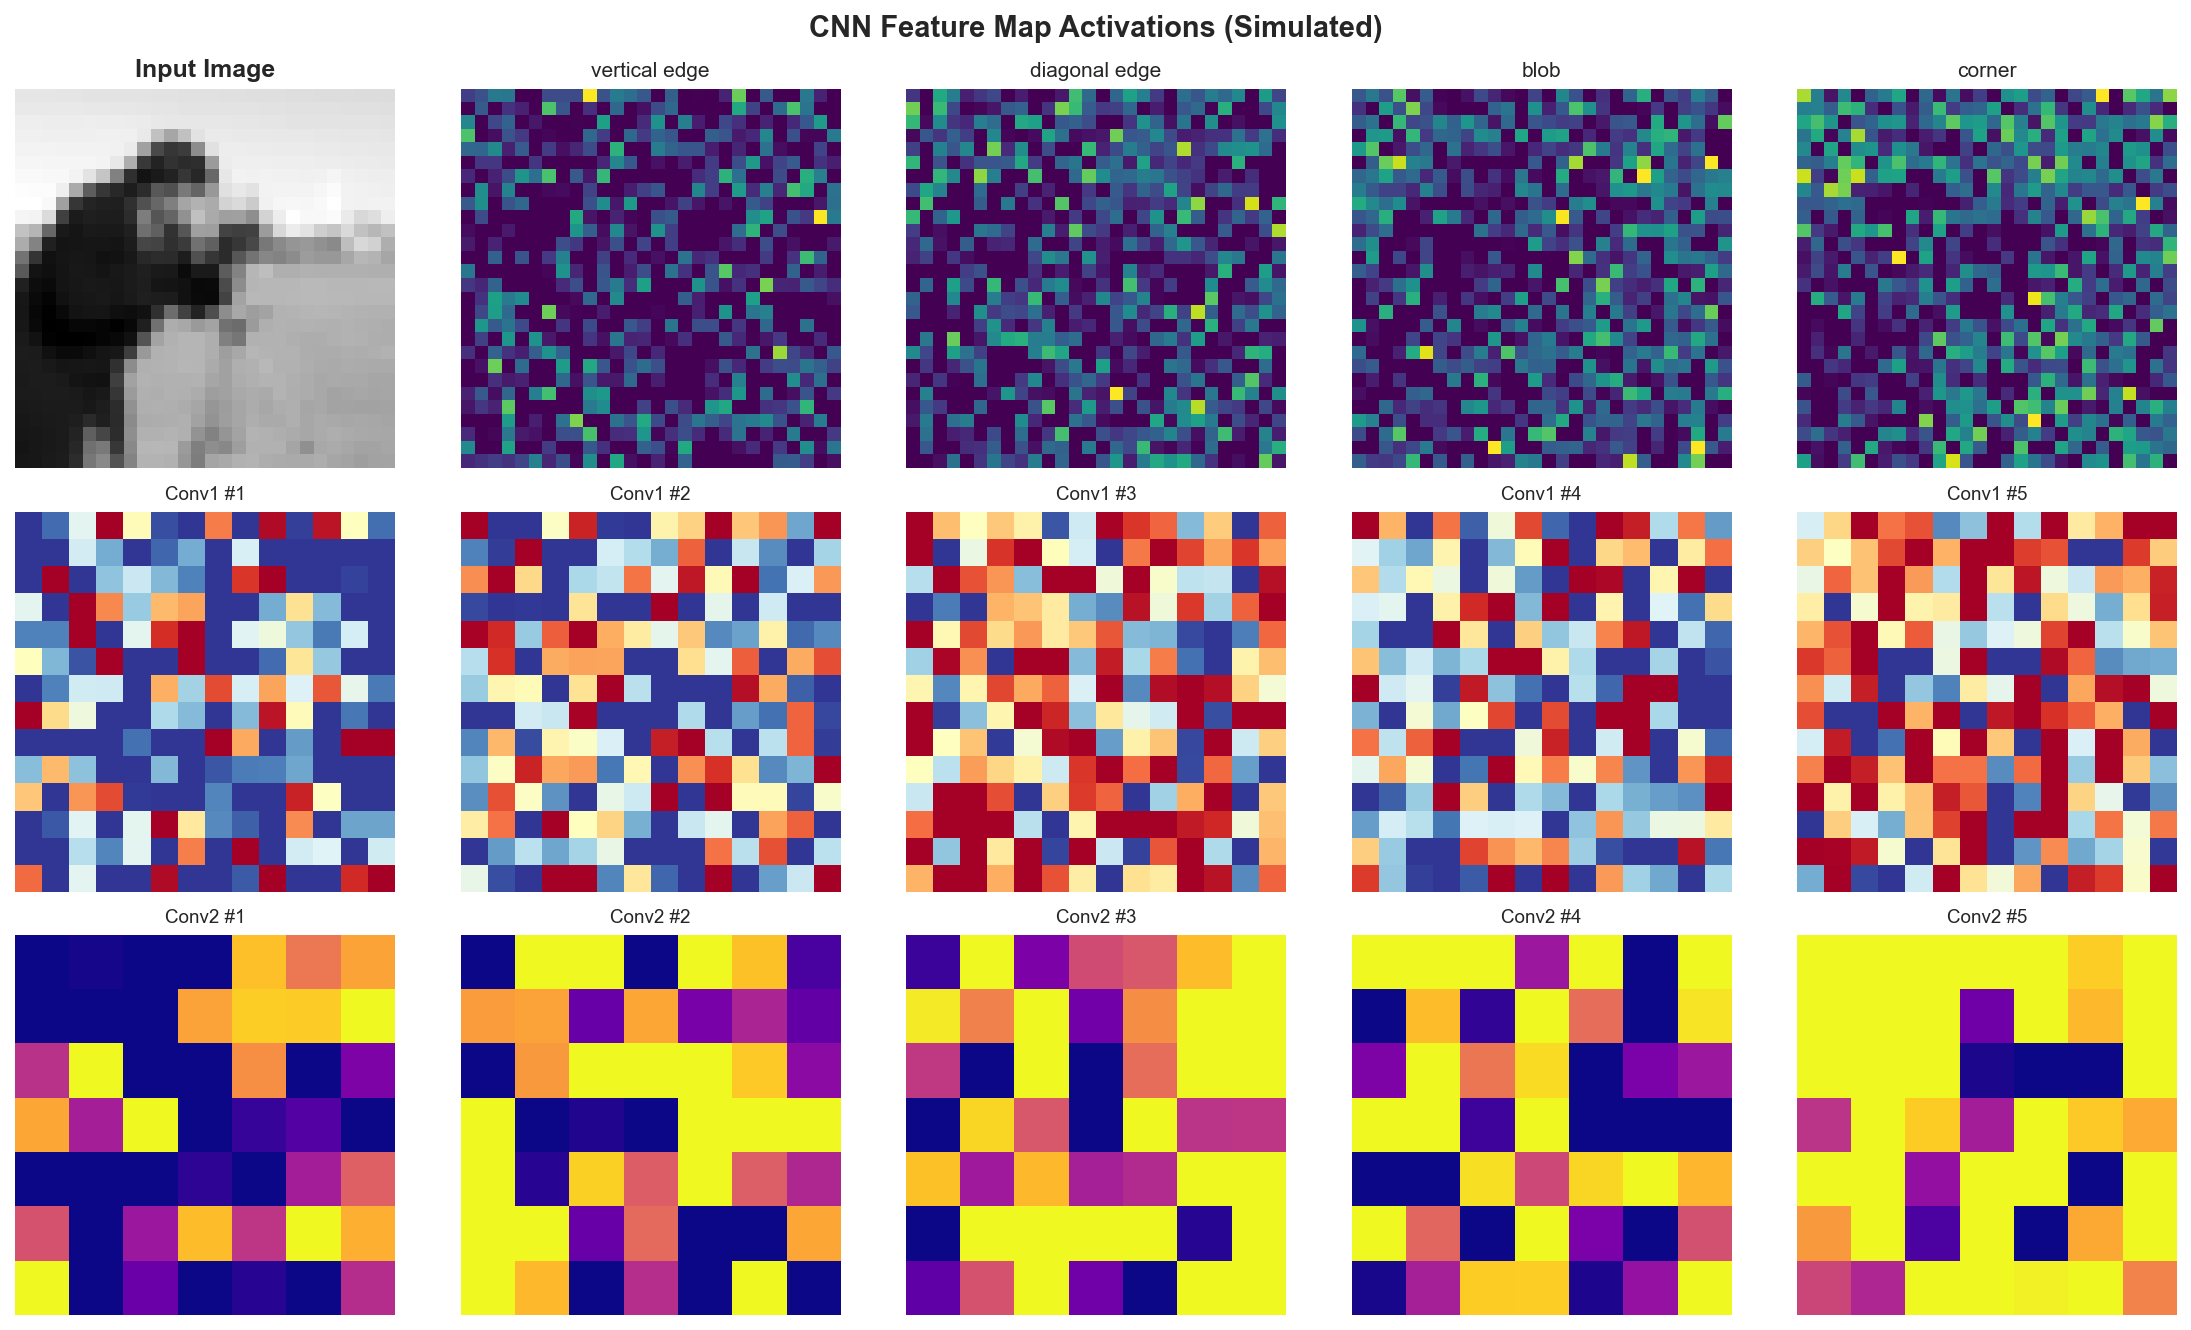
\includegraphics[width=0.7\textwidth]{../figures/feature_maps.png}
\end{center}

Early layers detect edges/textures, deeper layers learn complex patterns
\end{frame}

\begin{frame}{Training Image Classifiers}
\textbf{Loss Function:} Cross-entropy
\begin{equation}
\mathcal{L} = -\frac{1}{N}\sum_{i=1}^{N} \sum_{k=1}^{K} y_{ik} \log(\hat{y}_{ik})
\end{equation}

\textbf{Training:} Forward pass → Loss → Backprop → Update weights

\textbf{Key Hyperparameters:}
\begin{itemize}
\item Learning rate: $10^{-3}$ to $10^{-4}$, Batch: 32-128
\item Optimizer: SGD, Adam, RMSprop
\end{itemize}
\end{frame}

\begin{frame}{Training Curves}
\begin{center}
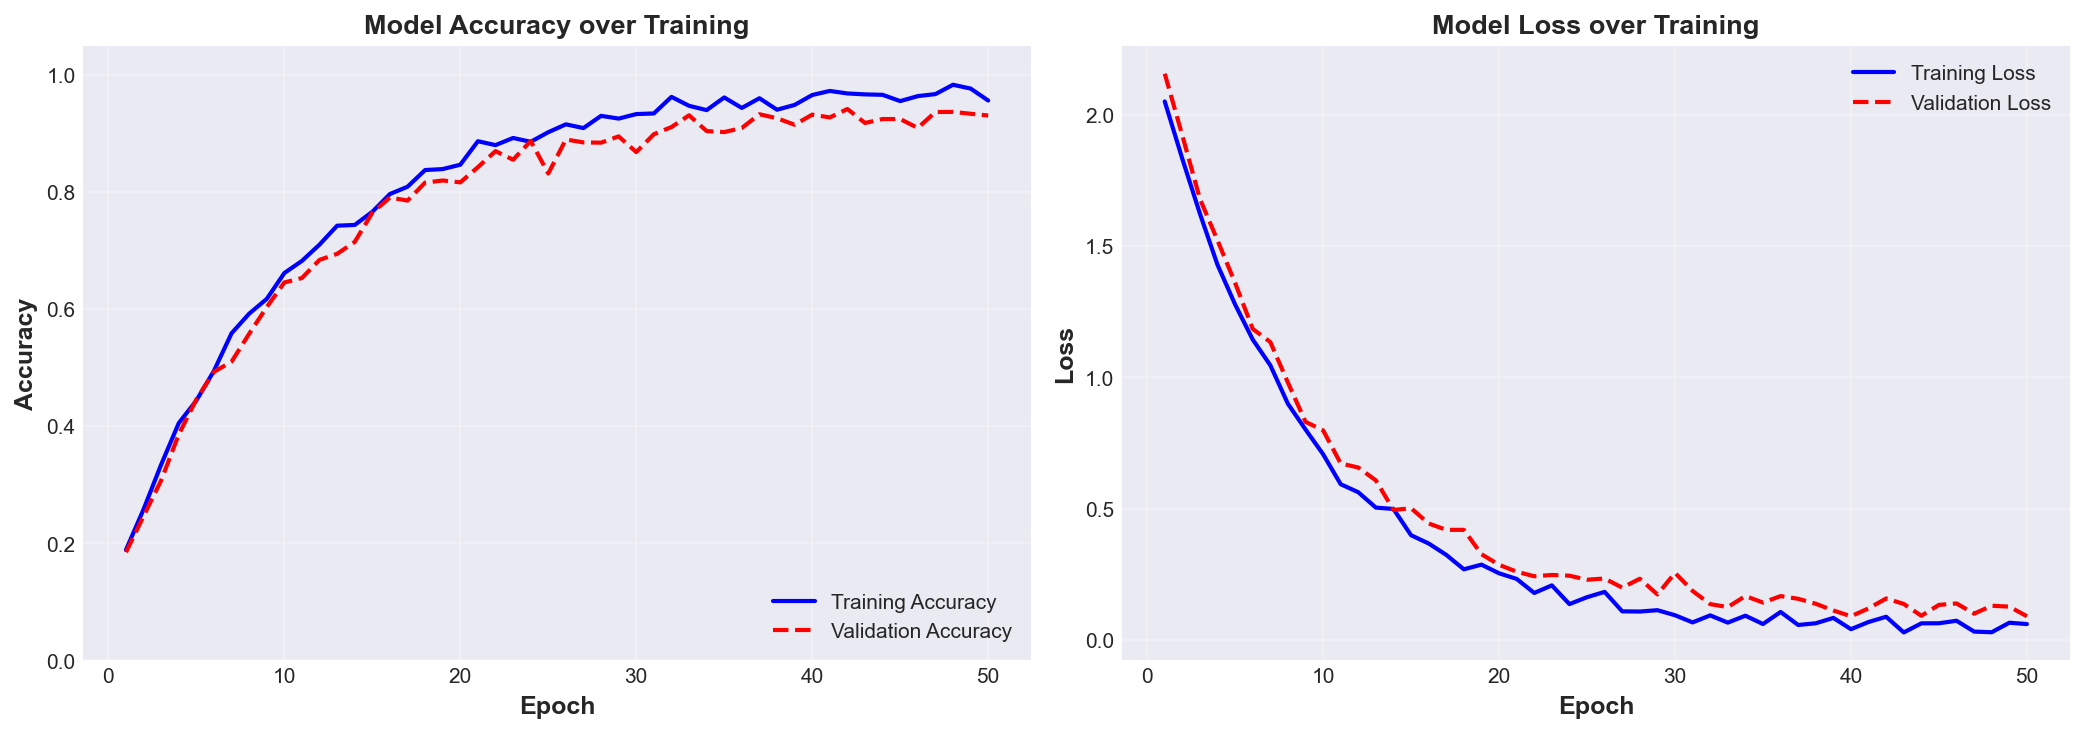
\includegraphics[width=0.85\textwidth]{../figures/training_curves.png}
\end{center}

\textbf{Monitoring:} Train accuracy ↑, val accuracy shows generalization, gap = overfitting
\end{frame}

\begin{frame}{Model Predictions}
\begin{center}
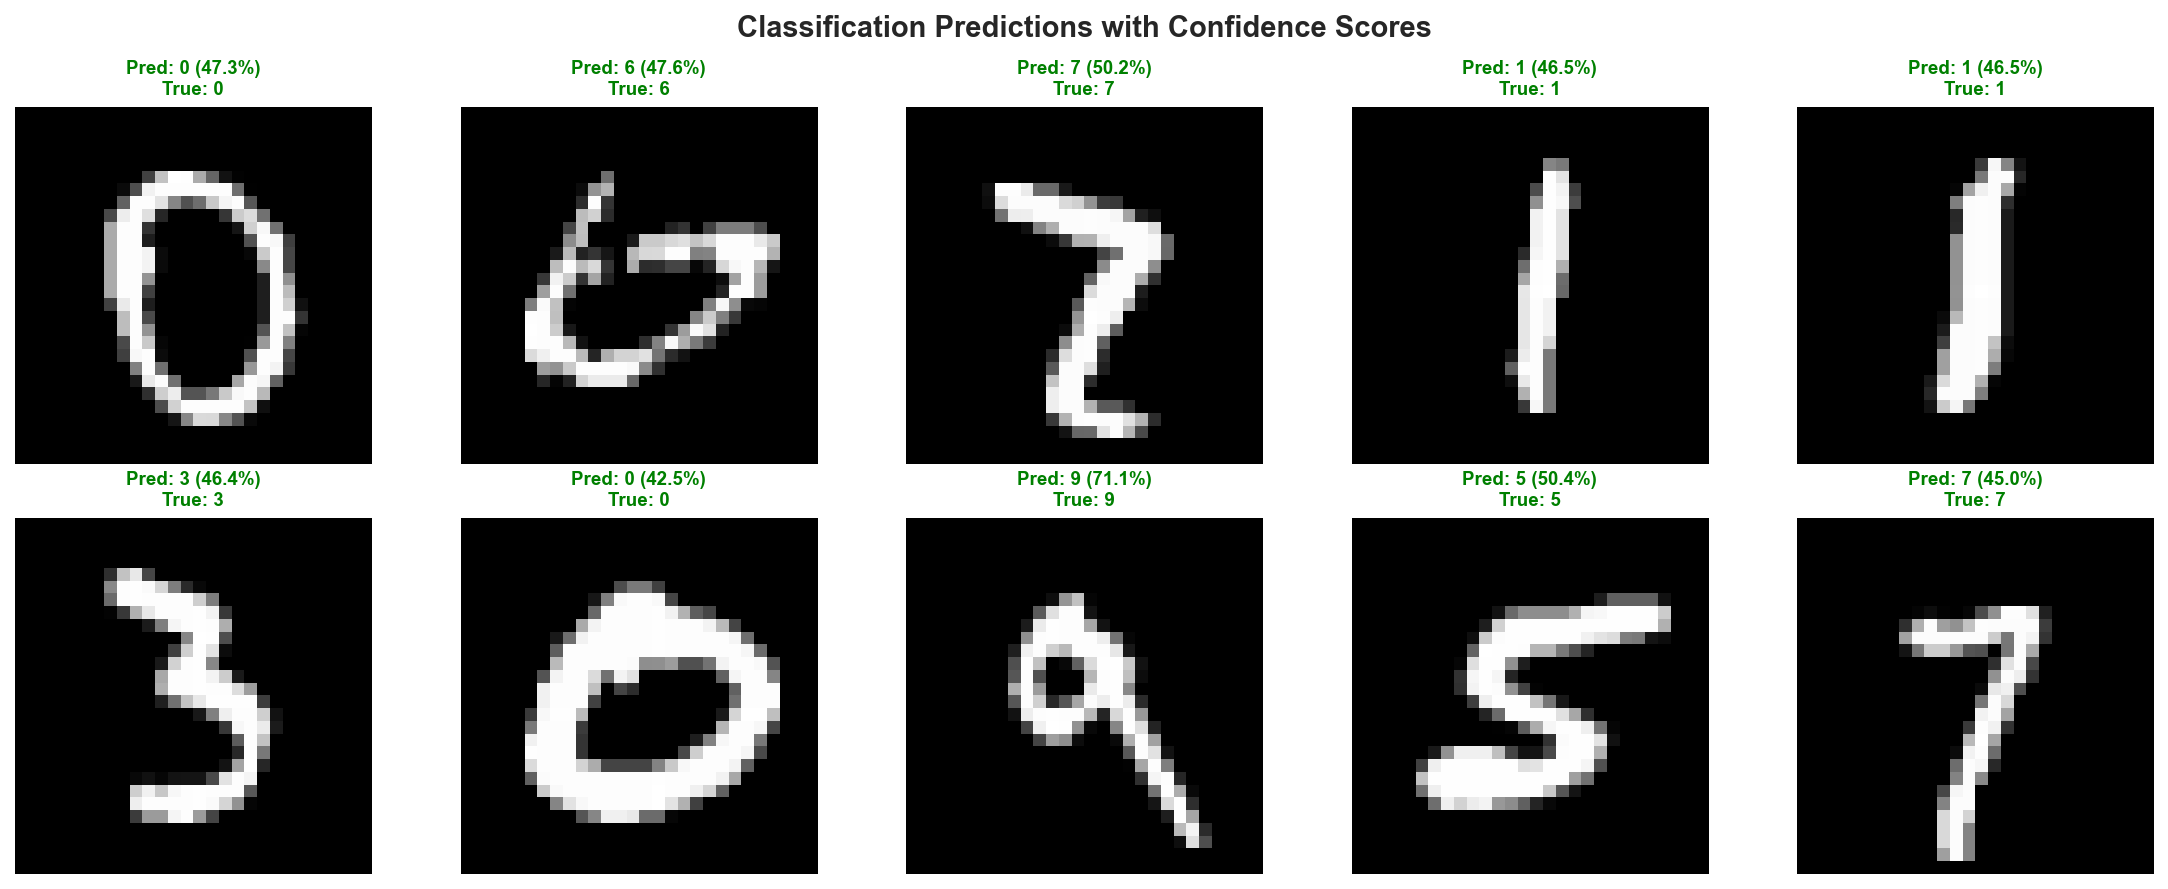
\includegraphics[width=0.85\textwidth]{../figures/multiclass_predictions.png}
\end{center}

\textbf{Analysis:} Confidence scores, correct vs incorrect predictions, border colors show accuracy
\end{frame}

\begin{frame}{Data Augmentation}
\textbf{Purpose:} Increase training data diversity and reduce overfitting

\textbf{Common Techniques:}
\begin{itemize}
\item \textbf{Geometric:} Rotation, flipping, translation, scaling
\item \textbf{Color:} Brightness, contrast, saturation adjustments
\item \textbf{Noise:} Gaussian noise, random erasing
\item \textbf{Advanced:} Cutout, Mixup, AutoAugment
\end{itemize}

\textbf{Implementation:}
\begin{itemize}
\item Apply transformations on-the-fly during training
\item Preserve label information
\item Use library functions (torchvision, Albumentations)
\end{itemize}
\end{frame}

\begin{frame}{Evaluation Metrics}
\begin{columns}
\column{0.5\textwidth}
\textbf{Key Metrics:}
\begin{itemize}
\item \textbf{Accuracy:} Overall correctness
\item \textbf{Precision:} True positives / predicted positives
\item \textbf{Recall:} True positives / actual positives
\item \textbf{F1 Score:} Harmonic mean of precision and recall
\end{itemize}

\textbf{Per-Class Analysis:}
\begin{itemize}
\item Confusion matrix visualization
\item Identify challenging classes
\item Class imbalance detection
\end{itemize}

\column{0.45\textwidth}
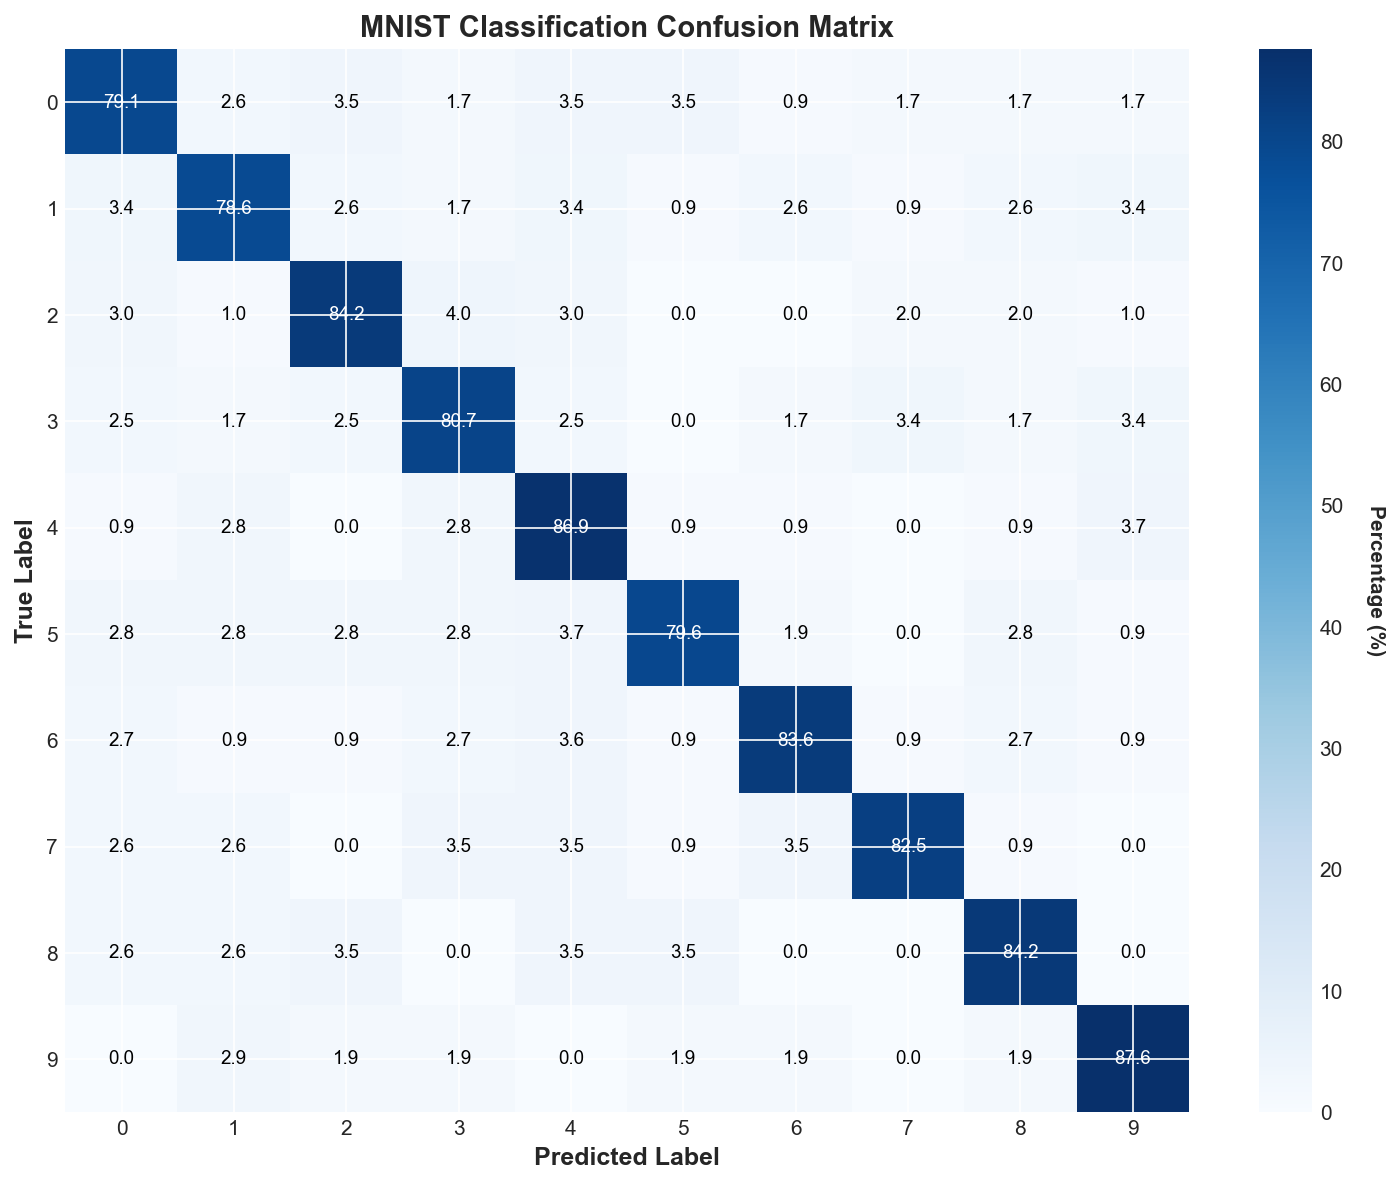
\includegraphics[width=\textwidth]{../figures/confusion_matrix.png}
\centering{\small Confusion matrix example}
\end{columns}
\end{frame}

\begin{frame}{Classic CNN Architectures}
\textbf{LeNet-5 (1998):}
\begin{itemize}
\item First successful CNN for digit recognition
\item 7 layers, pioneered conv-pool-fc structure
\end{itemize}

\textbf{AlexNet (2012):}
\begin{itemize}
\item ImageNet breakthrough, 8 layers
\item ReLU activation, dropout regularization
\end{itemize}

\textbf{VGGNet (2014):}
\begin{itemize}
\item Very deep (16-19 layers), small 3×3 filters
\item Demonstrated depth importance
\end{itemize}

\textbf{ResNet (2015):}
\begin{itemize}
\item Skip connections enable very deep networks (50-152 layers)
\item Solved vanishing gradient problem
\end{itemize}
\end{frame}

\section{Image Segmentation}

\begin{frame}{Segmentation Overview}
\begin{alertblock}{Definition}
Image segmentation partitions an image into multiple segments or regions, assigning a label to every pixel.
\end{alertblock}

\textbf{Segmentation Types:}
\begin{itemize}
\item \textbf{Semantic:} Classify each pixel by category
\item \textbf{Instance:} Distinguish individual objects
\item \textbf{Panoptic:} Combine semantic and instance
\end{itemize}

\textbf{Applications:}
\begin{itemize}
\item Medical imaging (tumor detection, organ segmentation)
\item Autonomous driving (road, pedestrian, vehicle detection)
\item Satellite imagery (land cover classification)
\item Video editing and AR/VR
\end{itemize}
\end{frame}

\begin{frame}{Semantic vs Instance Segmentation}
\begin{center}
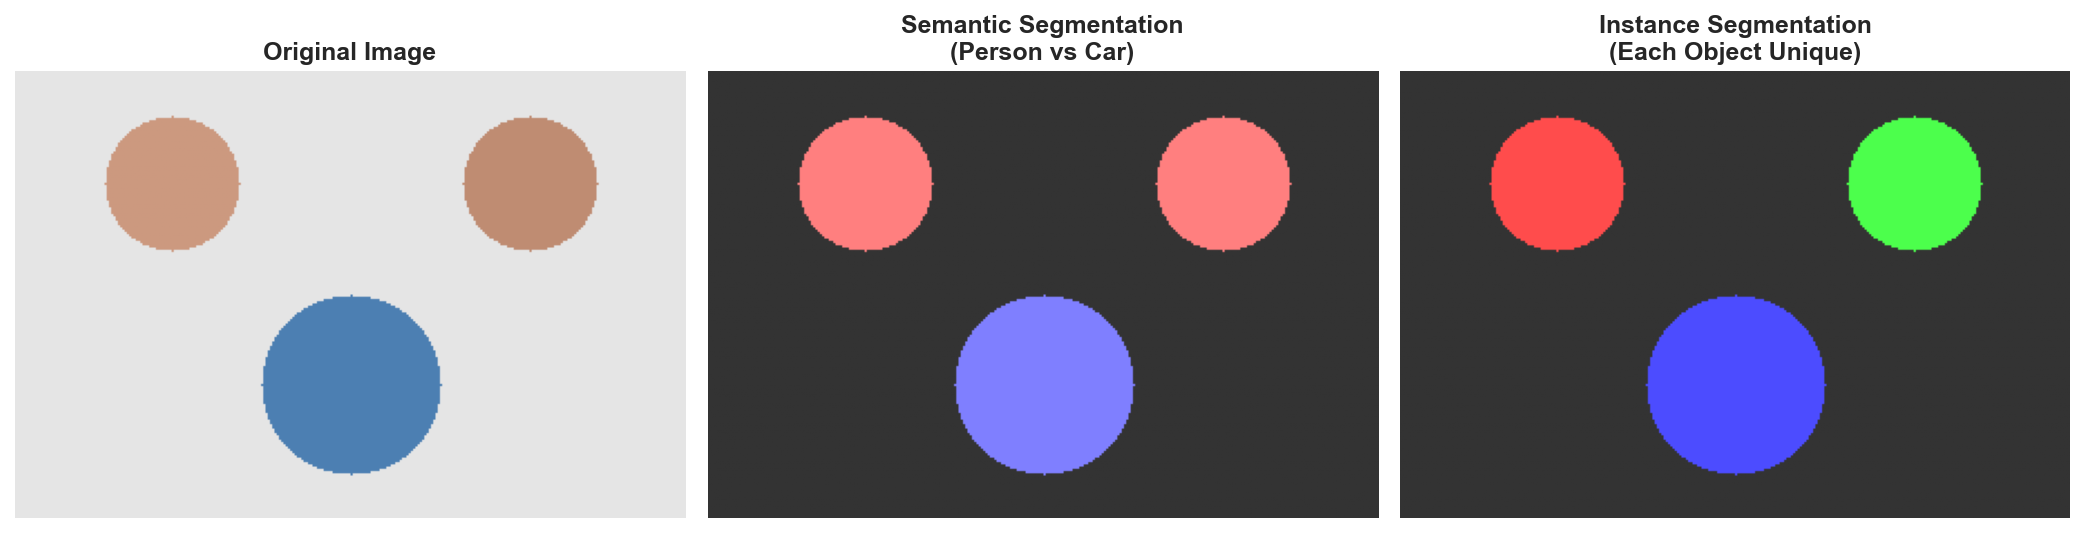
\includegraphics[width=0.95\textwidth]{../figures/segmentation_types.png}
\end{center}

\textbf{Key Differences:}
\begin{itemize}
\item \textbf{Semantic:} Same class → same label (all persons labeled "person")
\item \textbf{Instance:} Each object gets unique ID (person1, person2, ...)
\item Instance segmentation is more challenging but provides richer information
\end{itemize}
\end{frame}

\begin{frame}{U-Net Architecture}
\begin{center}
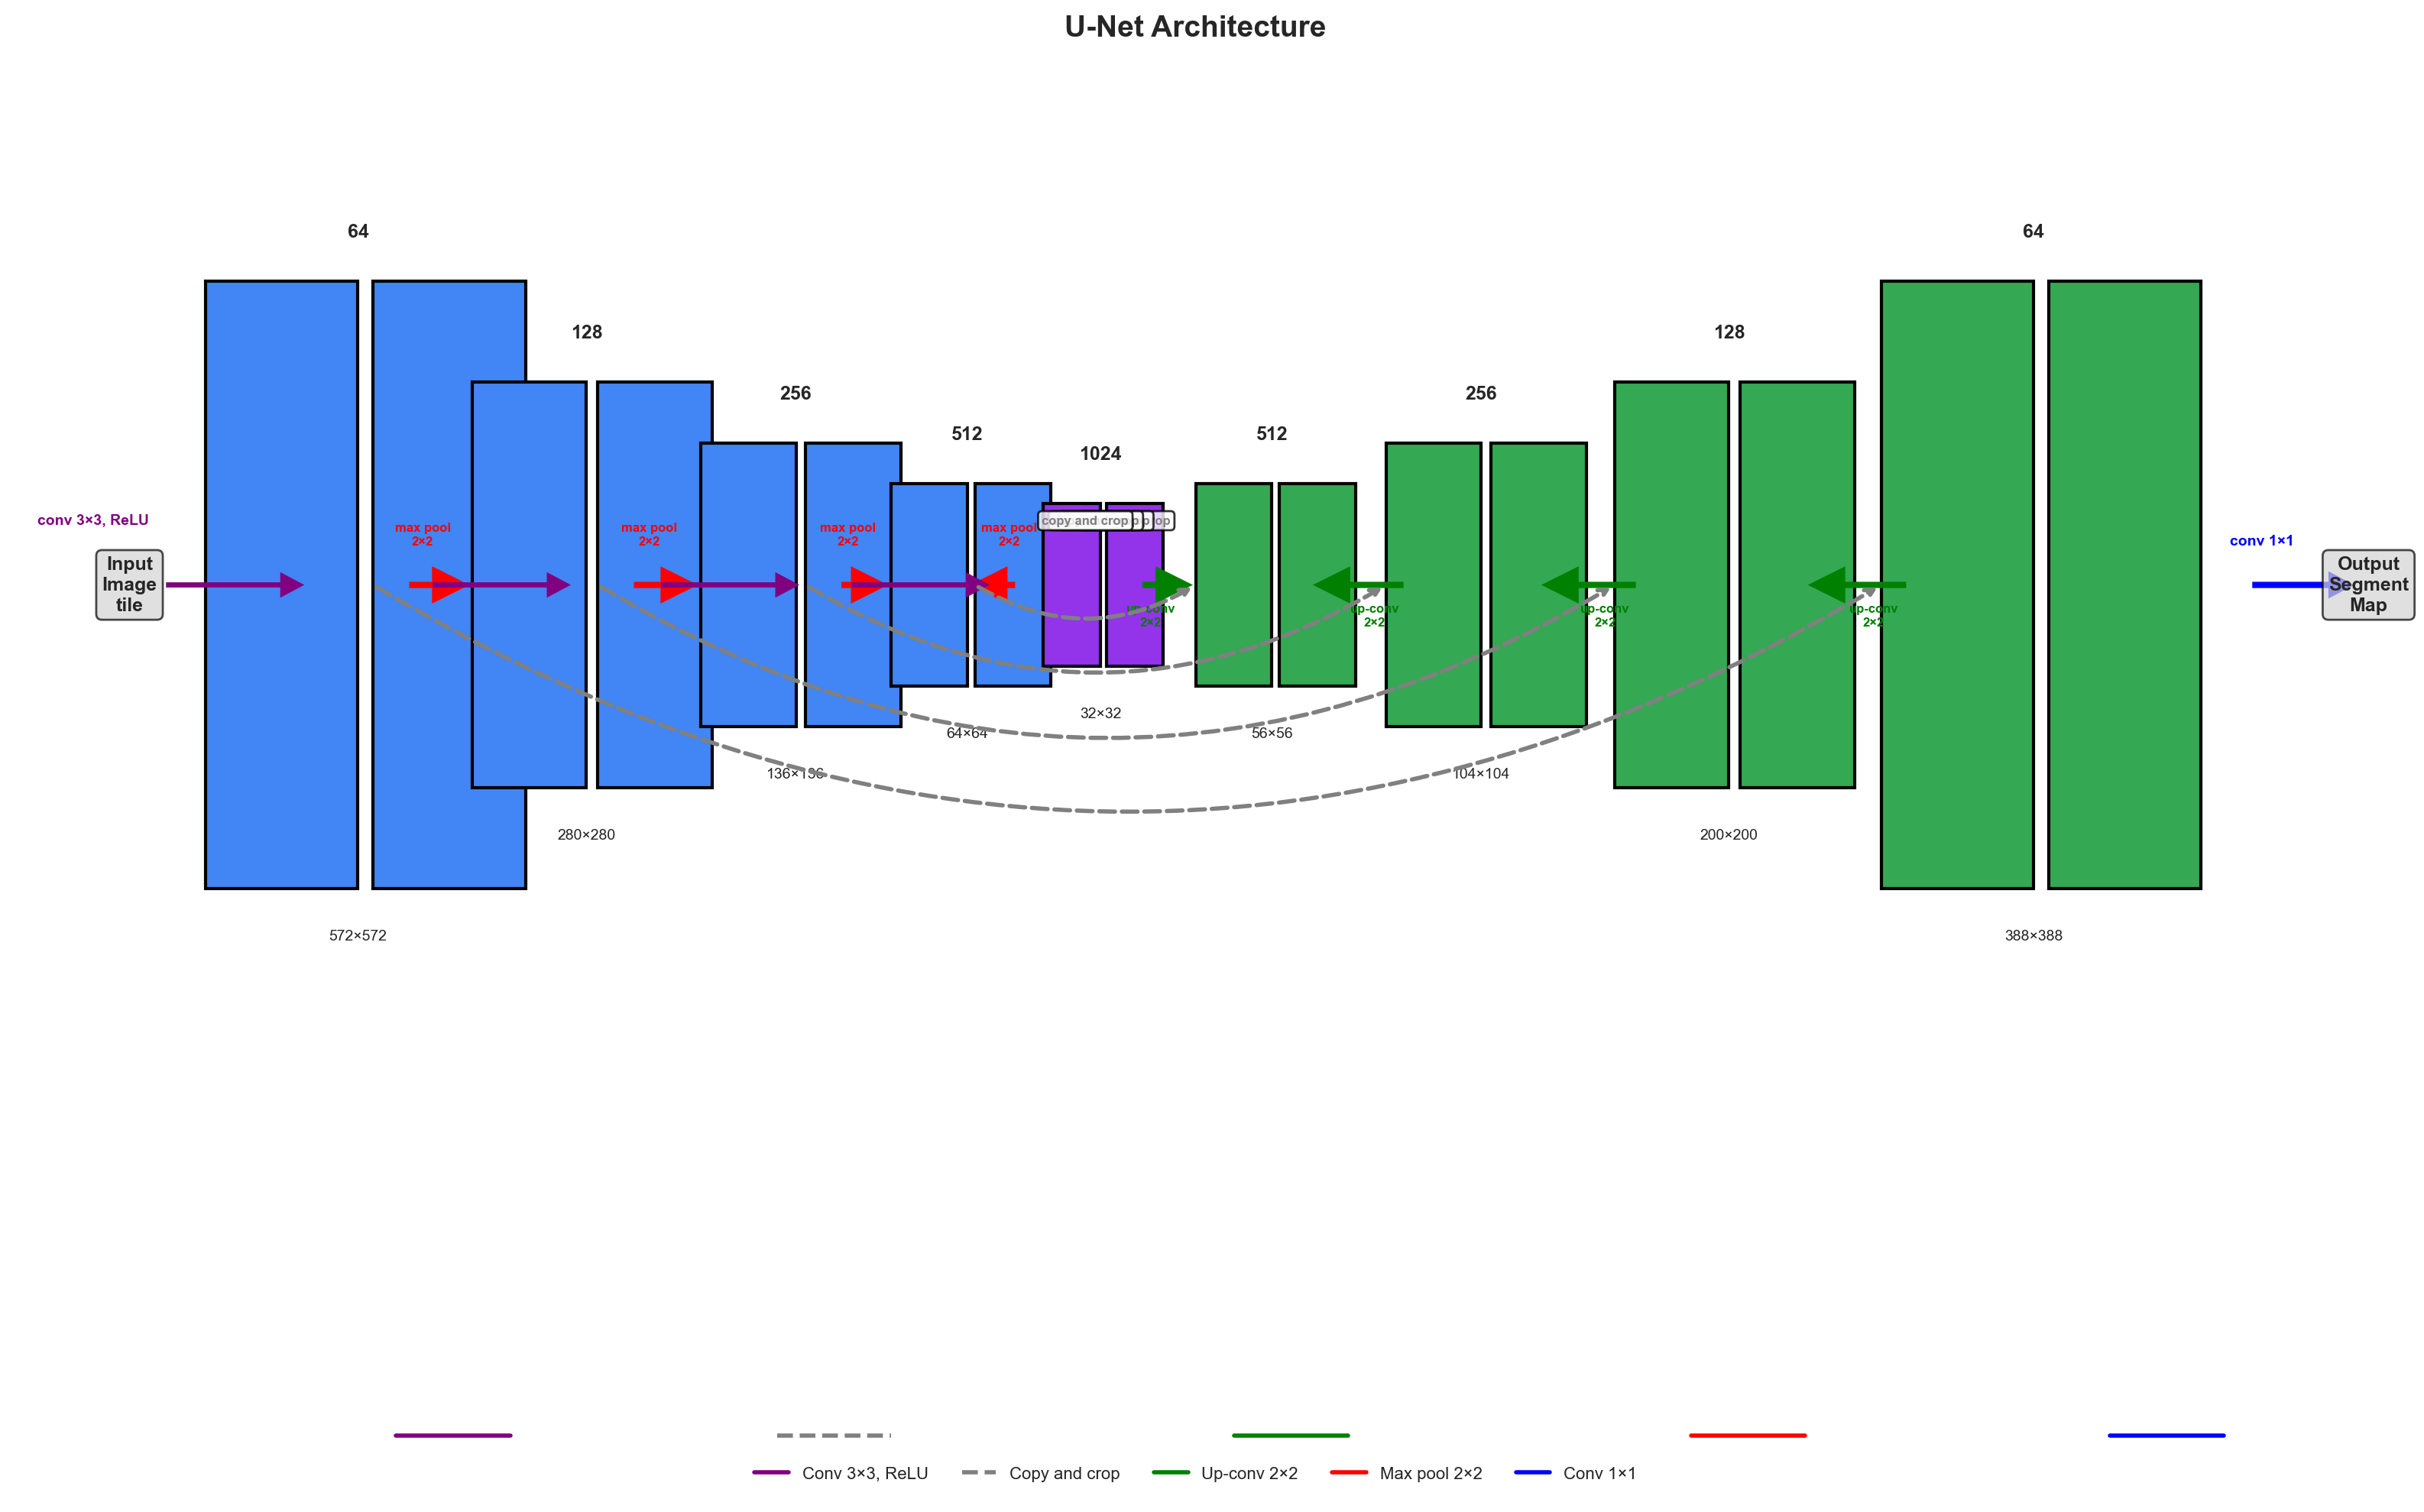
\includegraphics[width=0.72\textwidth]{../figures/unet_architecture.png}
\end{center}

Encoder-decoder + skip connections + symmetry
\end{frame}

\begin{frame}{U-Net Components}
\textbf{Encoder:} Conv + ReLU + pooling, doubles channels, halves resolution

\textbf{Decoder:} Upconv + concatenate encoder features (skip connections)

\textbf{Output:} 1×1 conv → pixel-wise softmax
\end{frame}

\begin{frame}{Segmentation Example}
\begin{center}
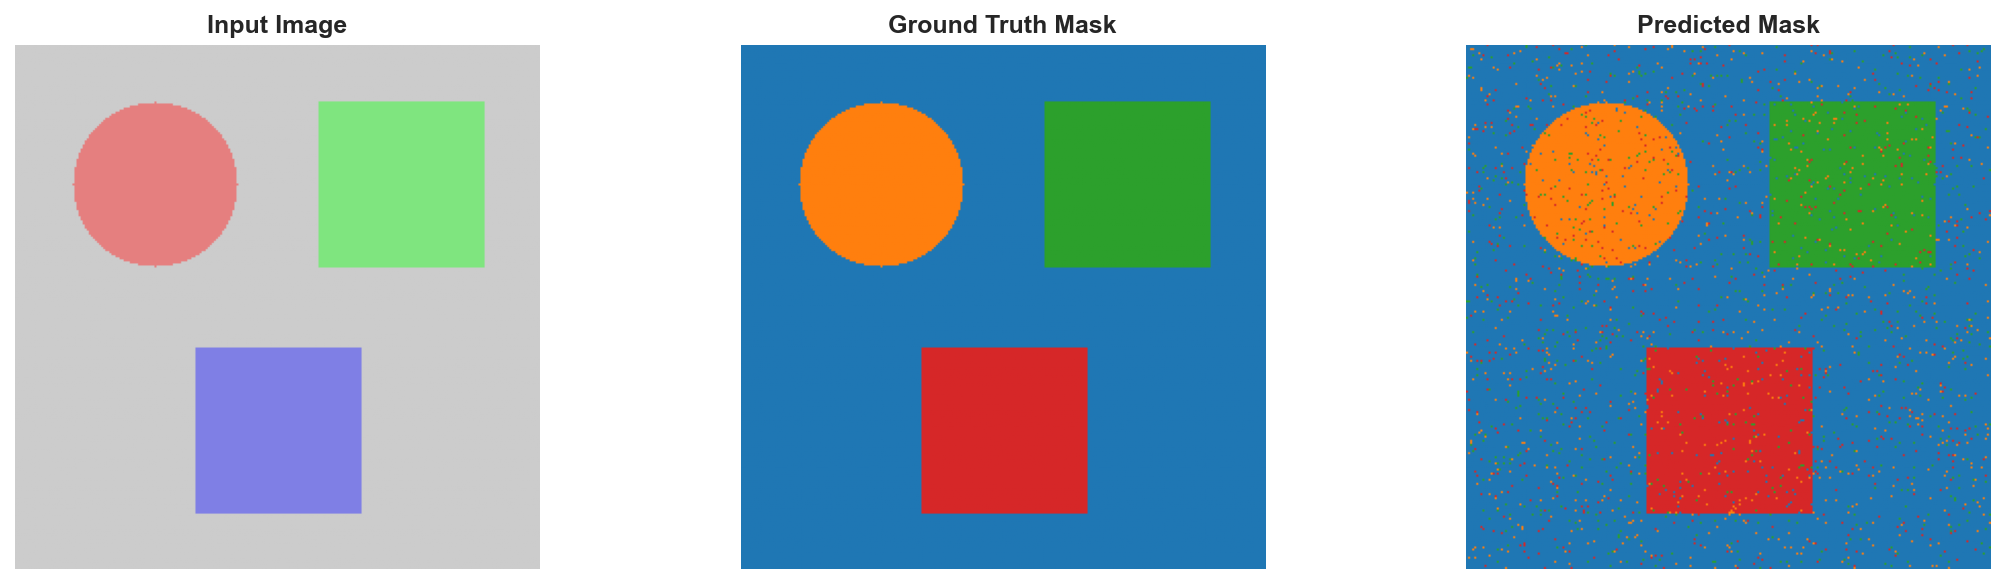
\includegraphics[width=0.95\textwidth]{../figures/segmentation_example.png}
\end{center}

\textbf{Workflow:}
\begin{enumerate}
\item Input image fed through network
\item Model predicts class for each pixel
\item Compare prediction with ground truth
\item Compute loss and update weights
\end{enumerate}
\end{frame}

\begin{frame}{Segmentation Loss Functions}
\textbf{Cross-Entropy Loss:}
\begin{equation}
\mathcal{L}_{CE} = -\frac{1}{N}\sum_{i=1}^{N} \sum_{c=1}^{C} y_{ic} \log(\hat{y}_{ic})
\end{equation}

\textbf{Dice Loss:}
\begin{equation}
\mathcal{L}_{Dice} = 1 - \frac{2 \sum_{i=1}^{N} p_i g_i}{\sum_{i=1}^{N} p_i + \sum_{i=1}^{N} g_i}
\end{equation}

\textbf{Choosing Loss:}
\begin{itemize}
\item Cross-entropy: Standard choice, class-balanced
\item Dice: Better for imbalanced data, small objects
\item Combined: Often use both for robustness
\end{itemize}
\end{frame}

\begin{frame}{Evaluation Metrics for Segmentation}
\begin{columns}
\column{0.5\textwidth}
\textbf{Intersection over Union (IoU):}
\begin{equation}
\text{IoU} = \frac{\text{Area of Overlap}}{\text{Area of Union}}
\end{equation}

\textbf{Mean IoU (mIoU):}
\begin{itemize}
\item Average IoU across all classes
\item Standard metric for segmentation
\item Range: [0, 1], higher is better
\end{itemize}

\column{0.45\textwidth}
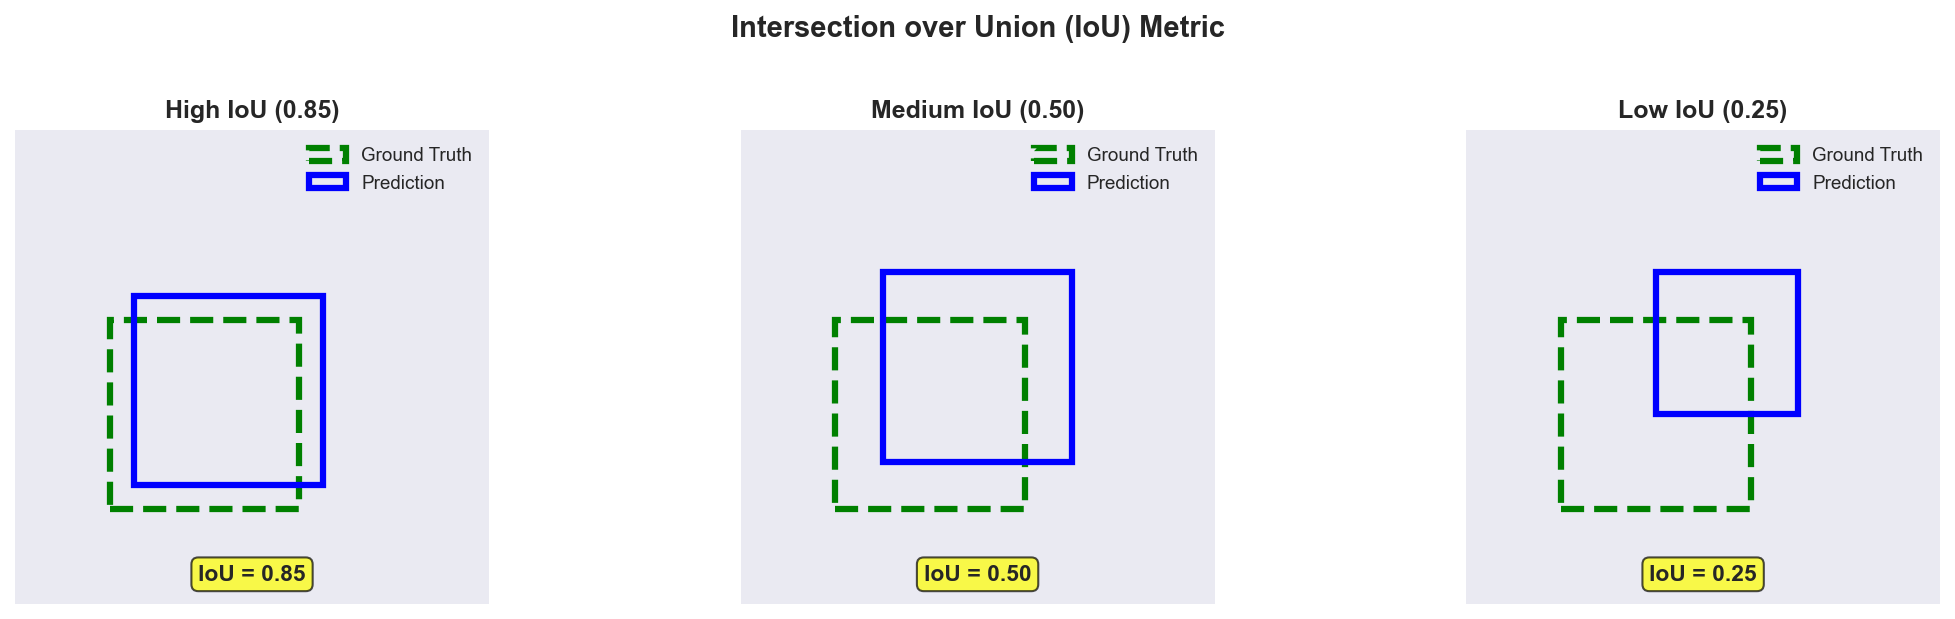
\includegraphics[width=\textwidth]{../figures/iou_visualization.png}
\centering{\small IoU examples}
\end{columns}
\end{frame}

\begin{frame}{Advanced Segmentation Architectures}
\textbf{FCN (Fully Convolutional Network):}
\begin{itemize}
\item First end-to-end CNN for segmentation
\item Replace FC layers with convolutions
\end{itemize}

\textbf{SegNet:}
\begin{itemize}
\item Encoder-decoder with pooling indices
\item Memory efficient upsampling
\end{itemize}

\textbf{DeepLab:}
\begin{itemize}
\item Atrous/dilated convolutions for larger receptive field
\item ASPP (Atrous Spatial Pyramid Pooling)
\end{itemize}

\textbf{Mask R-CNN:}
\begin{itemize}
\item Extends Faster R-CNN for instance segmentation
\item Adds mask prediction branch
\end{itemize}
\end{frame}

\section{Object Detection}

\begin{frame}{Object Detection Overview}
\begin{alertblock}{Definition}
Object detection identifies and localizes multiple objects in an image, providing both class labels and bounding box coordinates.
\end{alertblock}

\textbf{Output Format:}
\begin{itemize}
\item \textbf{Bounding box:} $(x, y, w, h)$ coordinates
\item \textbf{Class label:} Object category
\item \textbf{Confidence score:} Detection certainty
\end{itemize}

\textbf{Applications:}
\begin{itemize}
\item Autonomous vehicles (pedestrian, vehicle detection)
\item Surveillance and security systems
\item Retail (product recognition, inventory)
\item Robotics (object manipulation)
\end{itemize}
\end{frame}

\begin{frame}{Object Detection Example}
\begin{center}
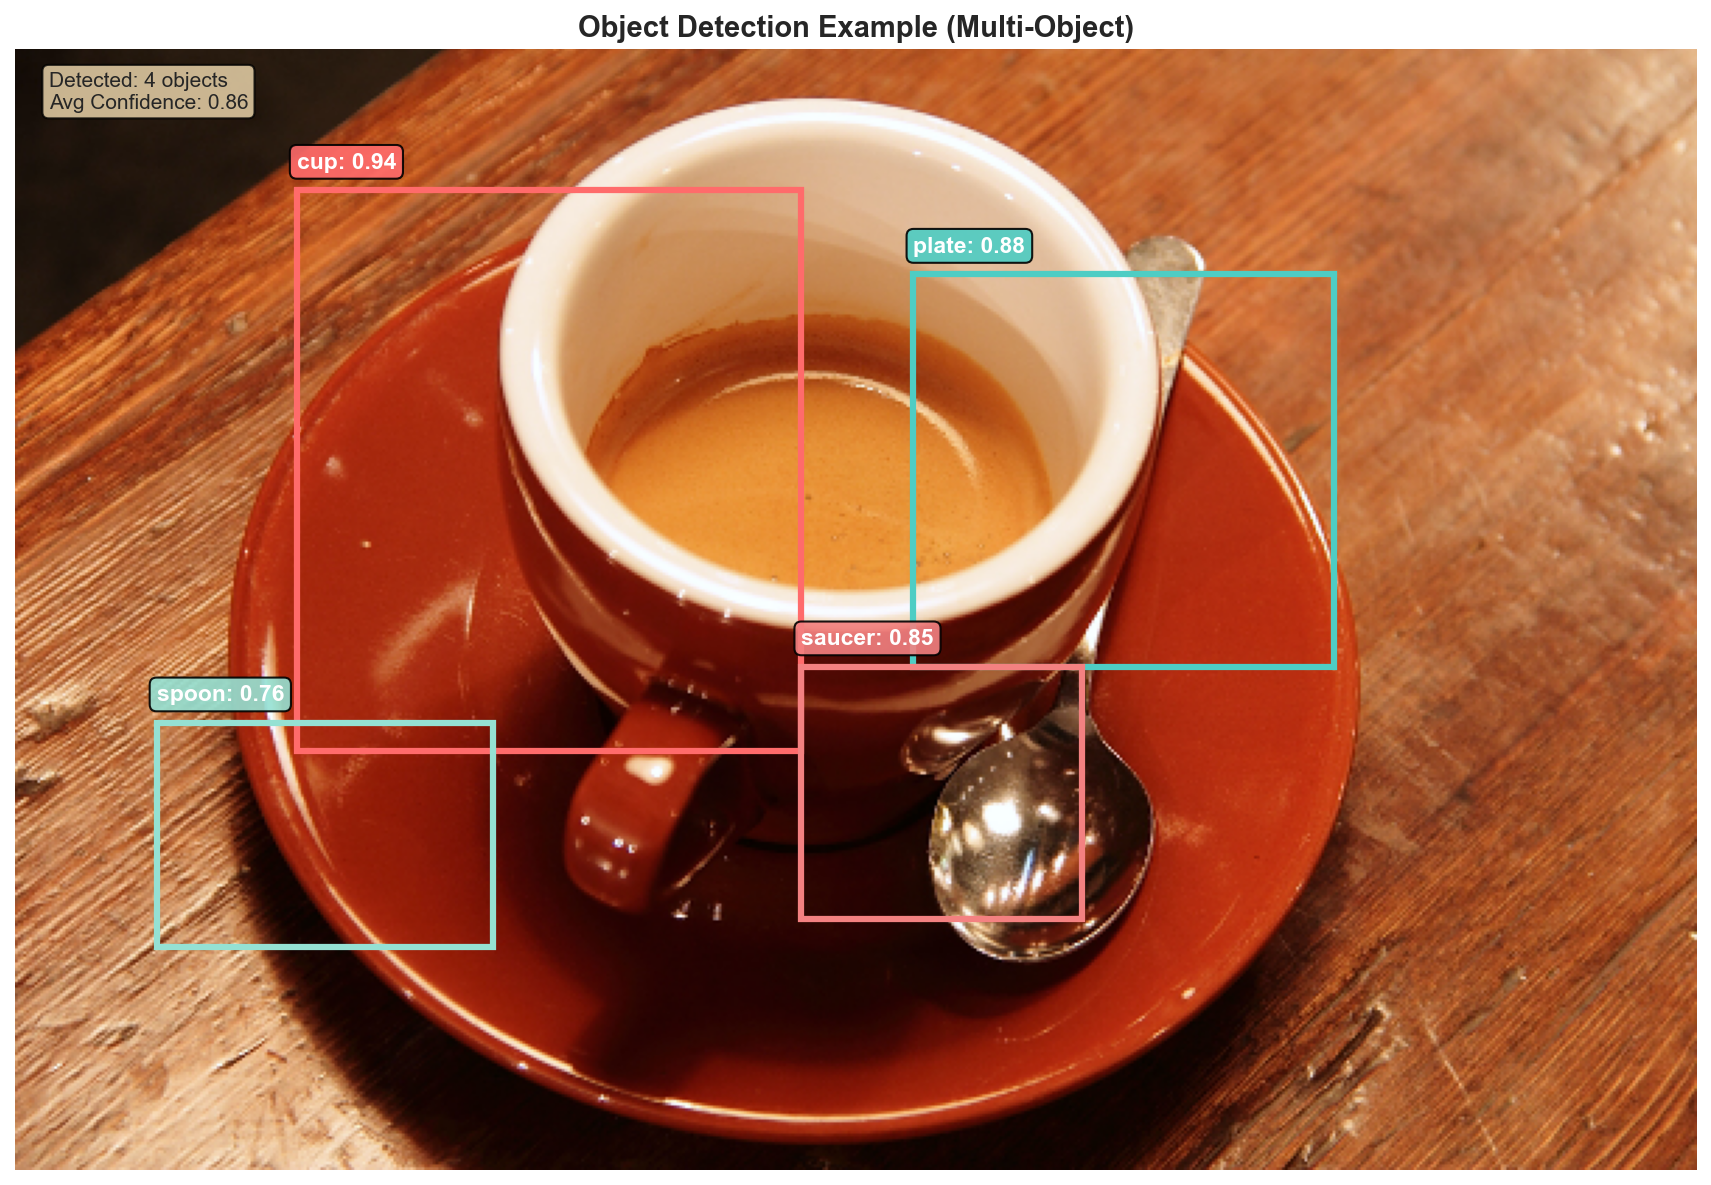
\includegraphics[width=0.65\textwidth]{../figures/detection_example.png}
\end{center}

\textbf{Challenges:} Variable count, scales, occlusion, real-time
\end{frame}

\begin{frame}{Two Approaches to Object Detection}
\textbf{Two-Stage Detectors:}
\begin{itemize}
\item Step 1: Generate region proposals
\item Step 2: Classify and refine proposals
\item Examples: R-CNN, Fast R-CNN, Faster R-CNN
\item Higher accuracy, slower inference
\end{itemize}

\textbf{One-Stage Detectors:}
\begin{itemize}
\item Direct prediction of boxes and classes
\item Single network pass
\item Examples: YOLO, SSD, RetinaNet
\item Faster inference, slightly lower accuracy
\end{itemize}
\end{frame}

\begin{frame}{R-CNN Family Evolution}
\textbf{R-CNN (2014):}
\begin{itemize}
\item Selective search for proposals (2000 per image)
\item CNN features + SVM classifier
\item Slow: 47s per image
\end{itemize}

\textbf{Fast R-CNN (2015):}
\begin{itemize}
\item Single CNN for entire image
\item RoI pooling for feature extraction
\item Faster: 2s per image
\end{itemize}

\textbf{Faster R-CNN (2015):}
\begin{itemize}
\item Region Proposal Network (RPN)
\item End-to-end trainable
\item Real-time capable: 0.2s per image
\end{itemize}
\end{frame}

\begin{frame}{Faster R-CNN Architecture}
\begin{center}
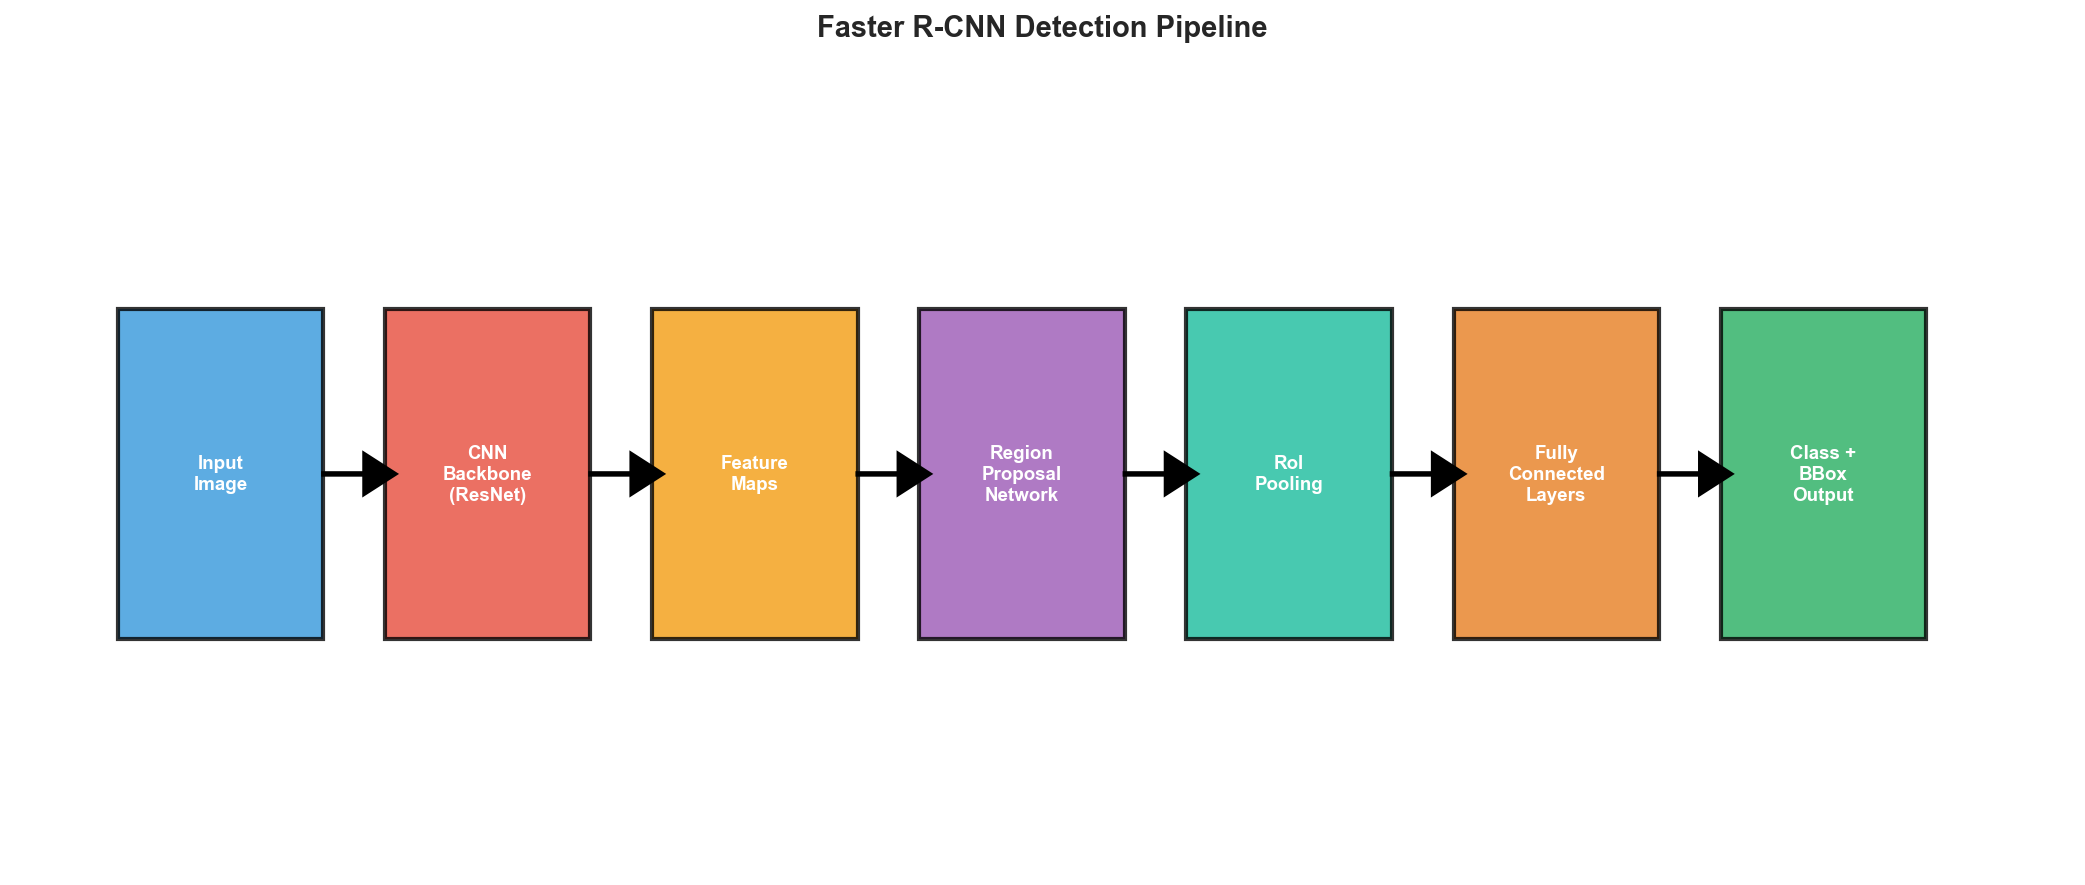
\includegraphics[width=0.9\textwidth]{../figures/faster_rcnn_pipeline.png}
\end{center}

\textbf{Pipeline:} CNN backbone → RPN → RoI pooling → Detection head
\end{frame}

\begin{frame}{Region Proposal Network (RPN)}
\textbf{Concept:} Slides over feature map, predicts objectness

\textbf{Anchor Boxes:} 9 per location (3 scales × 3 ratios)

\textbf{Outputs:} Objectness score + bbox offsets
\end{frame}

\begin{frame}{YOLO: You Only Look Once}
\begin{alertblock}{Key Idea}
YOLO treats detection as a single regression problem, directly predicting bounding boxes and class probabilities from full images in one evaluation.
\end{alertblock}

\textbf{Advantages:}
\begin{itemize}
\item Extremely fast: 45+ FPS on GPU
\item Global context (sees entire image)
\item Fewer false positives on background
\end{itemize}

\textbf{Architecture:}
\begin{itemize}
\item Divides image into $S \times S$ grid
\item Each cell predicts $B$ bounding boxes
\item Each box has: $(x, y, w, h, \text{confidence})$
\item Plus $C$ class probabilities per cell
\end{itemize}
\end{frame}

\begin{frame}{YOLO Grid-Based Detection}
\begin{center}
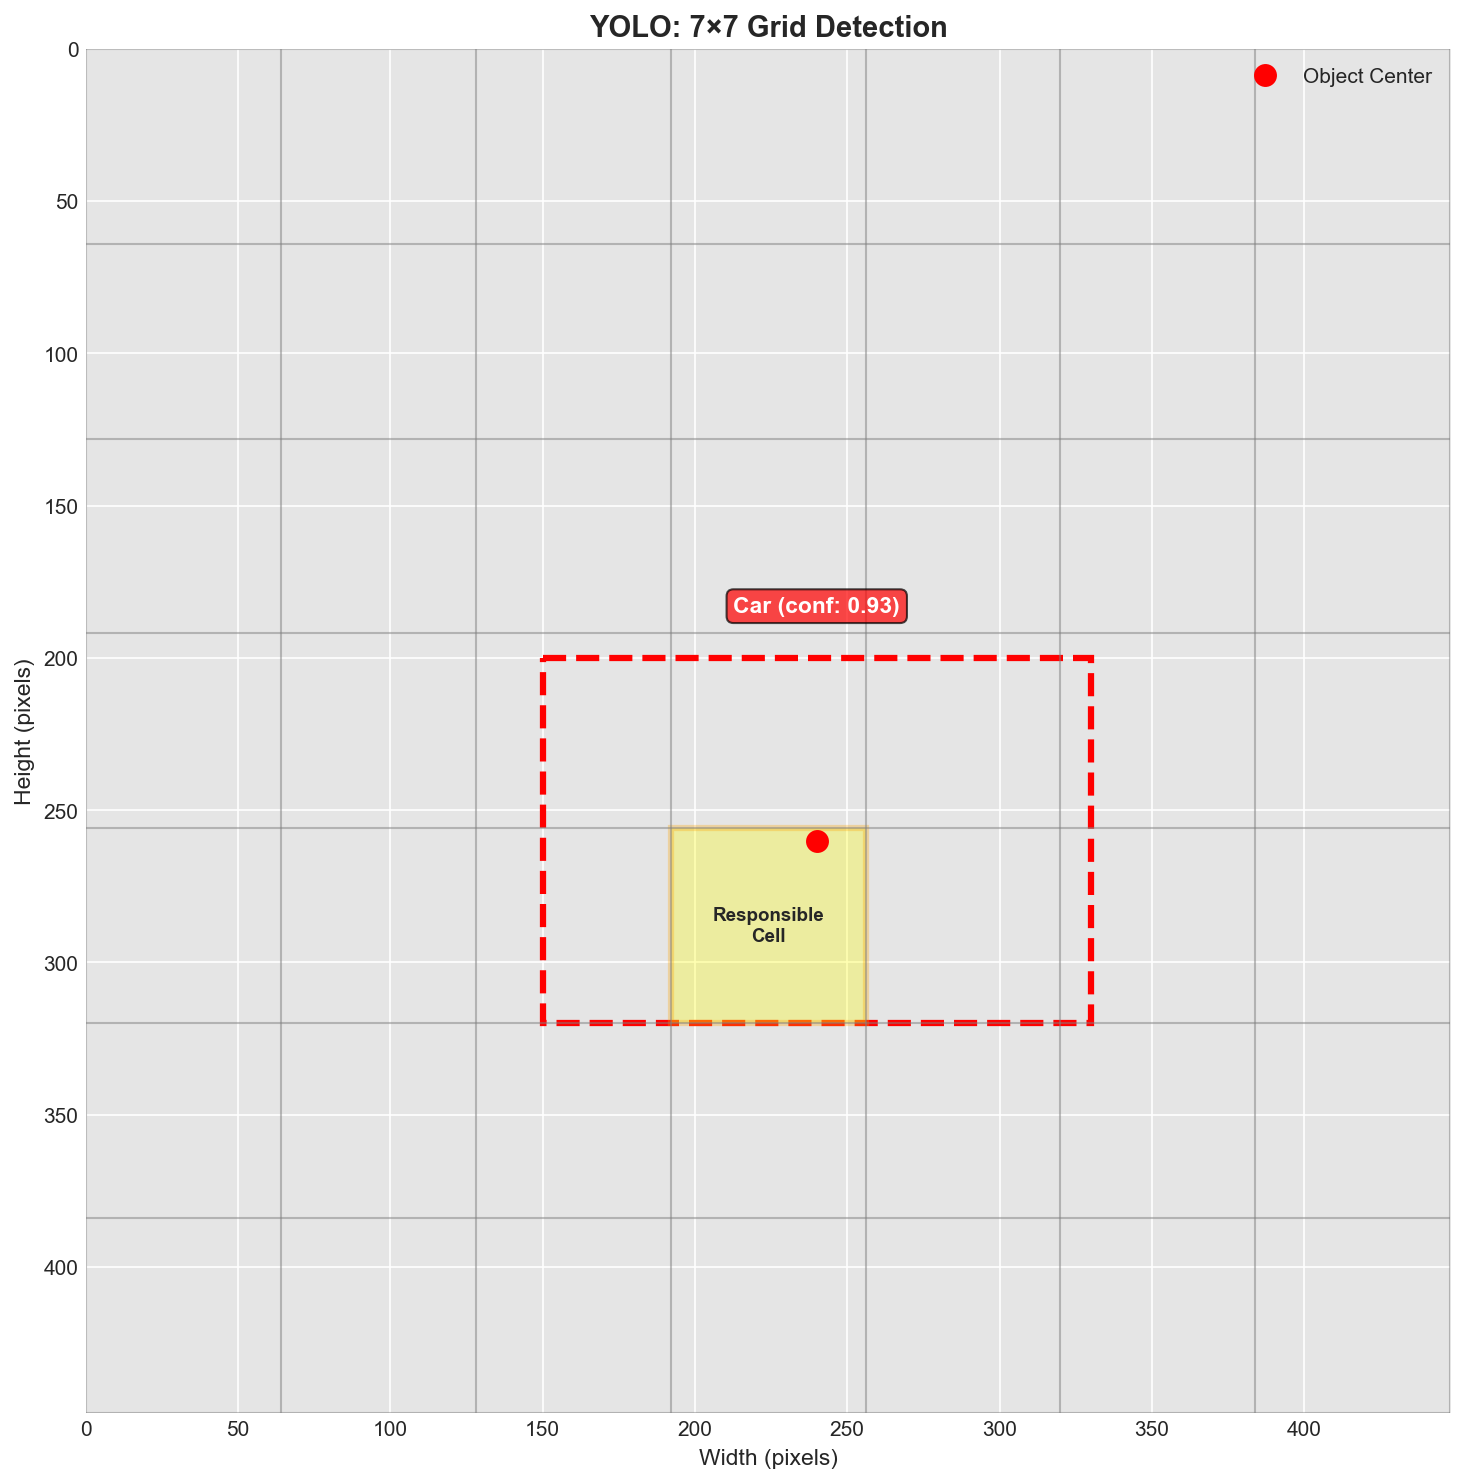
\includegraphics[width=0.45\textwidth]{../figures/yolo_grid.png}
\end{center}

Cell with object center predicts bbox + class
\end{frame}

\begin{frame}{YOLO Loss Function}
\small
\textbf{Multi-part Loss:}
\begin{equation}
\mathcal{L} = \lambda_{coord} \mathcal{L}_{loc} + \mathcal{L}_{conf} + \lambda_{noobj} \mathcal{L}_{noobj} + \mathcal{L}_{class}
\end{equation}

\textbf{Components:} Localization + confidence + classification

\textbf{Weights:} $\lambda_{coord} = 5$ (emphasize localization), $\lambda_{noobj} = 0.5$
\end{frame}

\begin{frame}{YOLO Versions}
\textbf{YOLOv1 (2016):}
\begin{itemize}
\item Original grid-based approach
\item 45 FPS, 63.4\% mAP on VOC
\end{itemize}

\textbf{YOLOv2/YOLO9000 (2017):}
\begin{itemize}
\item Batch normalization, anchor boxes
\item Multi-scale training
\end{itemize}

\textbf{YOLOv3 (2018):}
\begin{itemize}
\item Feature pyramid, better small object detection
\item Logistic regression for classes
\end{itemize}

\textbf{YOLOv4-v8 (2020-2023):}
\begin{itemize}
\item CSPNet backbone, advanced augmentation
\item State-of-the-art speed/accuracy trade-off
\end{itemize}
\end{frame}

\begin{frame}{Non-Maximum Suppression (NMS)}
\begin{center}
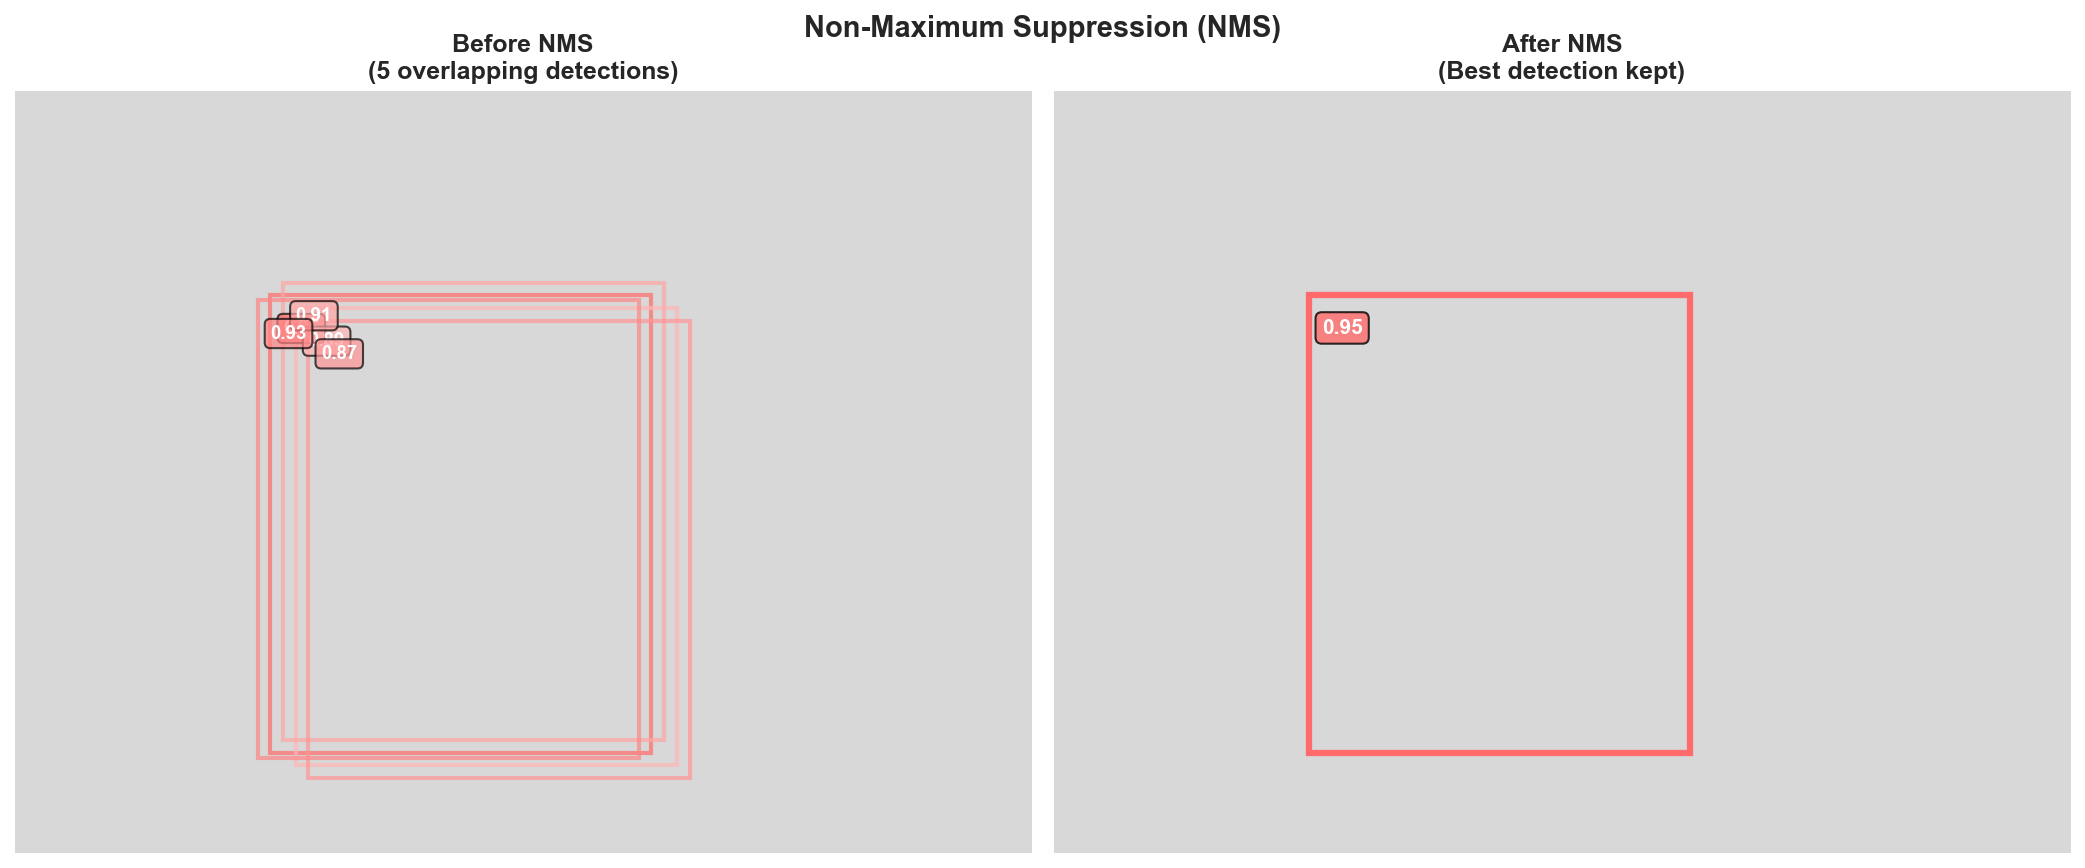
\includegraphics[width=0.8\textwidth]{../figures/nms_visualization.png}
\end{center}

\textbf{Goal:} Remove duplicate detections

\textbf{Method:} Sort by confidence, keep highest, remove overlaps (IoU $>$ threshold)
\end{frame}

\begin{frame}{Evaluation: Mean Average Precision (mAP)}
\begin{columns}
\column{0.5\textwidth}
\textbf{Average Precision (AP):}
\begin{itemize}
\item Area under precision-recall curve
\item Computed per class
\item Varies with IoU threshold
\end{itemize}

\textbf{Mean AP (mAP):}
\begin{equation}
\text{mAP} = \frac{1}{C} \sum_{c=1}^{C} \text{AP}_c
\end{equation}

\textbf{Standard Metrics:}
\begin{itemize}
\item mAP@0.5: IoU threshold 0.5
\item mAP@[0.5:0.95]: Average over multiple IoU thresholds
\end{itemize}

\column{0.45\textwidth}
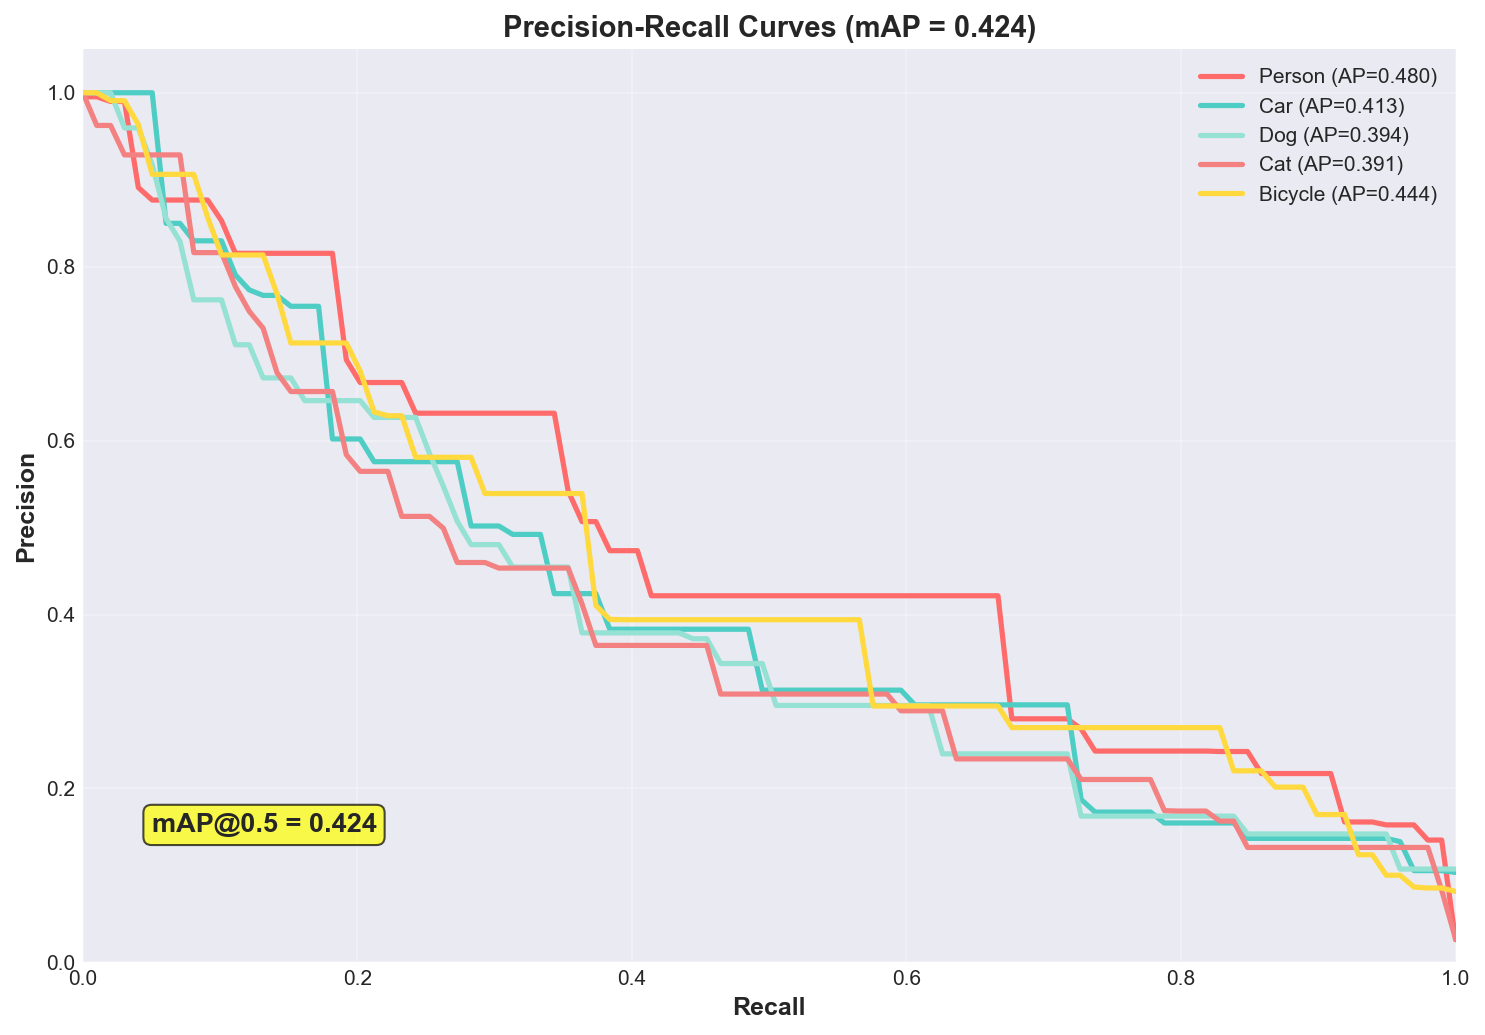
\includegraphics[width=\textwidth]{../figures/map_curve.png}
\centering{\small Precision-recall curves}
\end{columns}
\end{frame}

\begin{frame}{Detection Challenges}
\textbf{Scale Variation:}
\begin{itemize}
\item Objects appear at different sizes
\item Solution: Feature pyramids, multi-scale training
\end{itemize}

\textbf{Occlusion:}
\begin{itemize}
\item Objects partially hidden
\item Solution: Context modeling, attention mechanisms
\end{itemize}

\textbf{Class Imbalance:}
\begin{itemize}
\item Many more background samples
\item Solution: Focal loss, hard negative mining
\end{itemize}

\textbf{Real-time Constraints:}
\begin{itemize}
\item Need fast inference for applications
\item Solution: Lightweight backbones, pruning, quantization
\end{itemize}
\end{frame}

\section{Best Practices and Applications}

\begin{frame}{Transfer Learning}
\begin{alertblock}{Key Concept}
Transfer learning leverages pretrained models on large datasets (ImageNet) and fine-tunes them for specific tasks.
\end{alertblock}

\textbf{Advantages:}
\begin{itemize}
\item Faster training convergence
\item Better performance with limited data
\item Learned general features transfer well
\end{itemize}

\textbf{Strategies:}
\begin{itemize}
\item \textbf{Feature extraction:} Freeze early layers, train only classifier
\item \textbf{Fine-tuning:} Train entire network with small learning rate
\item \textbf{Progressive:} Gradually unfreeze layers during training
\end{itemize}
\end{frame}

\begin{frame}{Model Selection Guidelines}
\textbf{For Classification:}
\begin{itemize}
\item Small datasets: ResNet-18, MobileNet
\item Large datasets: ResNet-50/101, EfficientNet
\item Limited compute: SqueezeNet, MobileNetV3
\end{itemize}

\textbf{For Segmentation:}
\begin{itemize}
\item Medical imaging: U-Net, U-Net++
\item General purpose: DeepLabv3+, HRNet
\item Real-time: ENet, BiSeNet
\end{itemize}

\textbf{For Detection:}
\begin{itemize}
\item High accuracy: Faster R-CNN, Cascade R-CNN
\item Real-time: YOLOv5/v8, SSD
\item Mobile devices: MobileNet-SSD, YOLO-tiny
\end{itemize}
\end{frame}

\begin{frame}{Hyperparameter Tuning}
\textbf{Learning Rate:}
\begin{itemize}
\item Start: $10^{-3}$ to $10^{-4}$
\item Use learning rate finder or schedules
\item Cosine annealing, step decay
\end{itemize}

\textbf{Batch Size:}
\begin{itemize}
\item Larger batches: More stable, needs more memory
\item Smaller batches: Noisy gradients, regularization effect
\item Typical: 16-64 for detection, 32-128 for classification
\end{itemize}

\textbf{Regularization:}
\begin{itemize}
\item Dropout: 0.2-0.5 typical
\item Weight decay: $10^{-4}$ to $10^{-5}$
\item Early stopping based on validation loss
\end{itemize}
\end{frame}

\begin{frame}{Debugging Neural Networks - Part 1}
\textbf{Check Data Pipeline:}
\begin{itemize}
\item Visualize augmented samples
\item Verify label correctness
\item Check normalization statistics
\end{itemize}

\textbf{Monitor Training:}
\begin{itemize}
\item Plot loss curves (train and validation)
\item Track gradient magnitudes
\item Visualize predictions on validation set
\end{itemize}
\end{frame}

\begin{frame}{Debugging Neural Networks - Part 2}
\textbf{Overfit on Small Batch:}
\begin{itemize}
\item Try to overfit 1-10 samples
\item If fails, check architecture or learning rate
\end{itemize}

\textbf{Common Issues:}
\begin{itemize}
\item Exploding/vanishing gradients: Check initialization, use batch norm
\item Poor convergence: Adjust learning rate, check data quality
\item Overfitting: More data, stronger regularization, data augmentation
\end{itemize}
\end{frame}

\begin{frame}{Medical Imaging Application}
\textbf{Use Case:} Lung nodule detection in CT scans

\textbf{Approach:}
\begin{itemize}
\item U-Net for nodule segmentation
\item Transfer learning from ImageNet
\item Data augmentation: rotation, scaling, elastic deformation
\item Ensemble of models for robustness
\end{itemize}

\textbf{Challenges:}
\begin{itemize}
\item Class imbalance (few positive samples)
\item 3D volumetric data
\item High precision requirements
\item Limited labeled data
\end{itemize}
\end{frame}

\begin{frame}{Autonomous Driving Application}
\textbf{Use Case:} Multi-task perception system

\textbf{Tasks:}
\begin{itemize}
\item Object detection (pedestrians, vehicles, cyclists)
\item Lane segmentation
\item Drivable area segmentation
\item Traffic sign classification
\end{itemize}

\textbf{Architecture:}
\begin{itemize}
\item Shared backbone for efficiency
\item Multi-task learning with task-specific heads
\item Real-time inference ($>$30 FPS)
\end{itemize}
\end{frame}

\begin{frame}{Summary}
\textbf{Image Classification:}
\begin{itemize}
\item CNNs learn hierarchical features
\item Data augmentation and transfer learning are essential
\item Monitor training/validation curves
\end{itemize}

\textbf{Image Segmentation:}
\begin{itemize}
\item Pixel-wise classification for dense prediction
\item U-Net and encoder-decoder architectures
\item IoU and Dice metrics for evaluation
\end{itemize}

\textbf{Object Detection:}
\begin{itemize}
\item Two-stage (Faster R-CNN) vs one-stage (YOLO)
\item Trade-off between speed and accuracy
\item NMS and mAP for post-processing and evaluation
\end{itemize}
\end{frame}

\begin{frame}{Key Takeaways}
\begin{alertblock}{Important Points}
Deep learning has revolutionized computer vision, but success requires careful attention to data quality, architecture selection, and training procedures.
\end{alertblock}

\textbf{Best Practices:}
\begin{itemize}
\item Start with pretrained models (transfer learning)
\item Use data augmentation extensively
\item Monitor validation metrics to prevent overfitting
\item Select architecture based on task requirements
\item Iterate on data quality and model design
\end{itemize}
\end{frame}

\begin{frame}[standout]
Questions?
\end{frame}

\end{document}
